\section{二代测序数据分析}
\subsection{常见术语}
\begin{frame}
  \frametitle{基因组学 | 数据分析 | 术语 | \textcolor{red}{深度 vs. 覆盖度}}
  \begin{block}{深度(depth)}
    \begin{itemize}
      \item 也叫乘数,衡量测序量的首要参数;测序得到的总碱基数与待测基因组大小的比值;每个碱基被测序的平均次数
      \item 假设一个基因大小为2M,测序获得的总数据量为20M测序,那么深度为10X
    \end{itemize}
  \end{block}
  \pause
  \begin{block}{覆盖度(coverage)}
    \begin{itemize}
      \item 测序获得的序列占整个基因组的比例
      \item 由于基因组中的高GC、重复序列等复杂结构的存在,测序最终拼接组装获得的序列往往无法覆盖所有的区域,这部分没有获得的区域就称为Gap。例如一个细菌基因组测序,覆盖度是98\%,那么还有2\%的序列区域是没有通过测序获得的。
    \end{itemize}
  \end{block}
\end{frame}

\begin{frame}
  \frametitle{基因组学 | 数据分析 | 术语 | 深度 vs. 覆盖度}
  \begin{block}{实验}
对长100bp的目标区域进行捕获测序:采用单端测序,每个read长5bp;总共得到了200个reads;把所有的reads比对到目标区域后,100bp的目标区域中有98bp的位置至少有1个read覆盖到,换言之,剩余的2bp没有1个read覆盖。
  \end{block}
  \pause
  \begin{block}{深度与覆盖度}
    \begin{itemize}
      \item 深度:$200 \times 5 / 100 = 10$
      \item 覆盖度:$98 / 100 \times 100\% = 98\%$
    \end{itemize}
  \end{block}
\end{frame}

\begin{frame}
  \frametitle{基因组学 | 数据分析 | 术语 | SE vs. PE}
  \begin{figure}
    \centering
    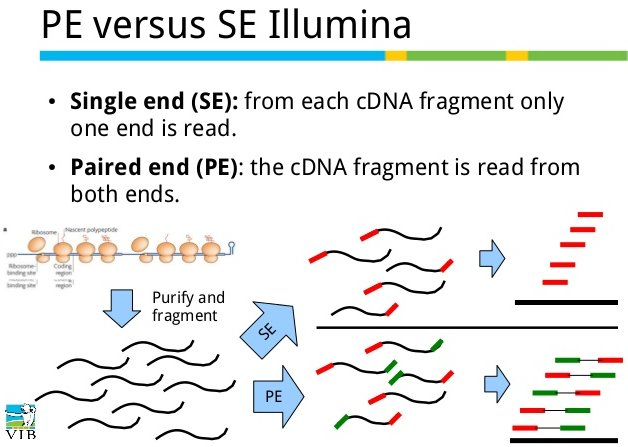
\includegraphics[width=0.85\textwidth]{c2.genomics/term.se.pe.01.jpg}
  \end{figure}
\end{frame}

\begin{frame}
  \frametitle{基因组学 | 数据分析 | 术语 | SE vs. PE}
  \begin{figure}
    \centering
    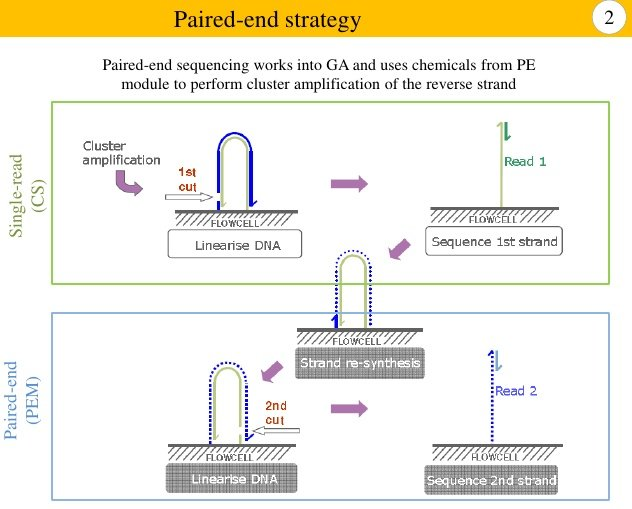
\includegraphics[width=0.8\textwidth]{c2.genomics/term.se.pe.02.jpg}
  \end{figure}
\end{frame}

\begin{frame}
  \frametitle{基因组学 | 数据分析 | 术语 | PE}
  \begin{block}{Paired-End Sequencing}
    \begin{itemize}
      \item allows users to sequence both ends of a fragment and generate high-quality, alignable sequence data
      \item facilitates detection of genomic rearrangements and repetitive sequence elements, as well as gene fusions and novel transcripts
    \end{itemize}
  \end{block}
  \begin{figure}
    \centering
    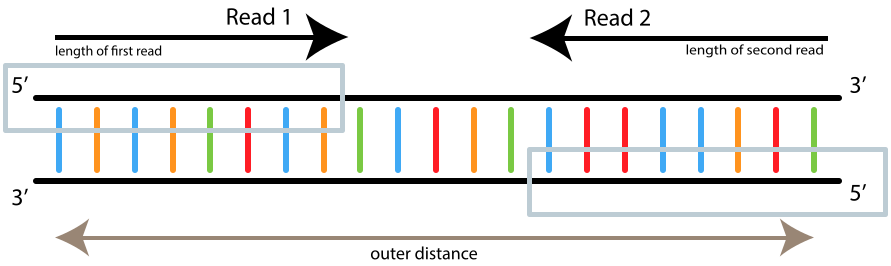
\includegraphics[width=0.9\textwidth]{c2.genomics/term.pe.01.png}
  \end{figure}
\end{frame}

\begin{frame}
  \frametitle{基因组学 | 数据分析 | 术语 | PE}
  \begin{block}{Paired-End DNA Sequencing}
    \begin{itemize}
      \item provide superior alignment across DNA regions containing repetitive sequences
      \item produce longer contigs for de novo sequencing by filling gaps in the consensus sequence
      \item detect rearrangements such as insertions, deletions, and inversions
    \end{itemize}
  \end{block}
  \pause
  \begin{block}{Paired-End RNA Sequencing}
    \begin{itemize}
      \item enable discovery applications such as detecting gene fusions in cancer and characterizing novel splice isoforms.
    \end{itemize}
  \end{block}
\end{frame}

\begin{frame}
  \frametitle{基因组学 | 数据分析 | 术语 | \textcolor{red}{PE}}
  \begin{figure}
    \centering
    \only<1->{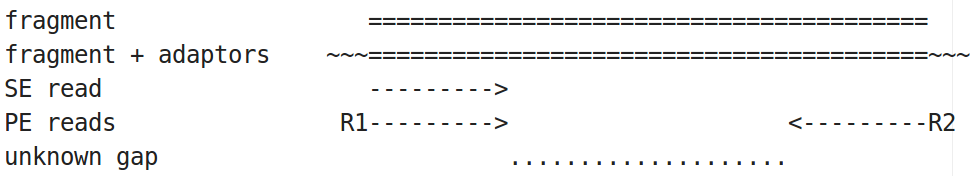
\includegraphics[width=\textwidth]{c2.genomics/term.insert.size.01.png}}\\
    \vspace{1em}
    \only<2->{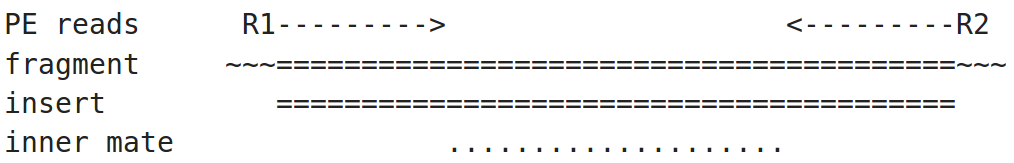
\includegraphics[width=\textwidth]{c2.genomics/term.insert.size.02.png}}
  \end{figure}
  \only<3->{
  \begin{block}{Conclusion}
Remember that ``insert" refers to the DNA fragment between the adaptors, and not the gap between R1 and R2. Instead we refer to that as the ``inner mate distance".
  \end{block}
  }
\end{frame}

\begin{frame}
  \frametitle{基因组学 | 数据分析 | 术语 | \textcolor{red}{其他}}
  \begin{figure}
    \centering
    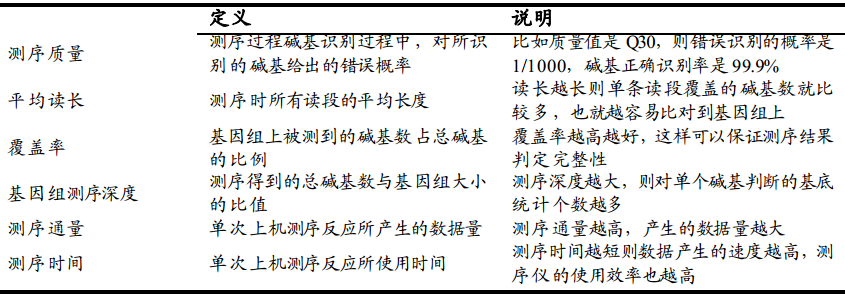
\includegraphics[width=\textwidth]{c2.genomics/term.other.01.png}
  \end{figure}
\end{frame}

\subsection{分析流程}
\begin{frame}
  \frametitle{基因组学 | 数据分析 | 流程 | 概述 | 总览}
  \begin{figure}
    \centering
    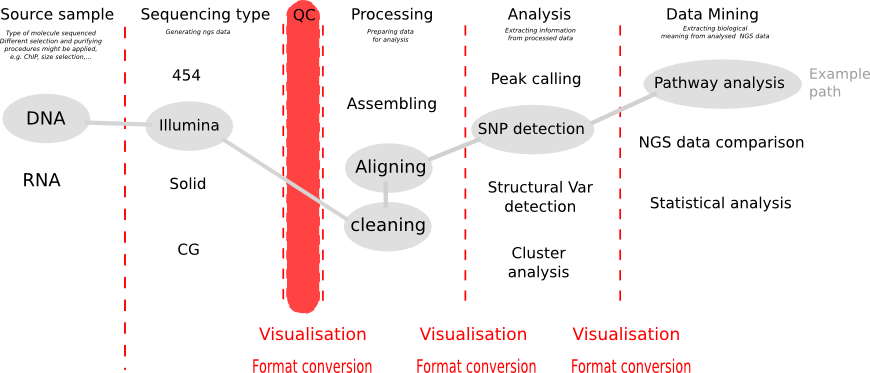
\includegraphics[width=\textwidth]{c2.genomics/workflow.ngs.05.png}
  \end{figure}
\end{frame}

\begin{frame}
  \frametitle{基因组学 | 数据分析 | 流程 | 概述 | 总览}
  \begin{figure}
    \centering
    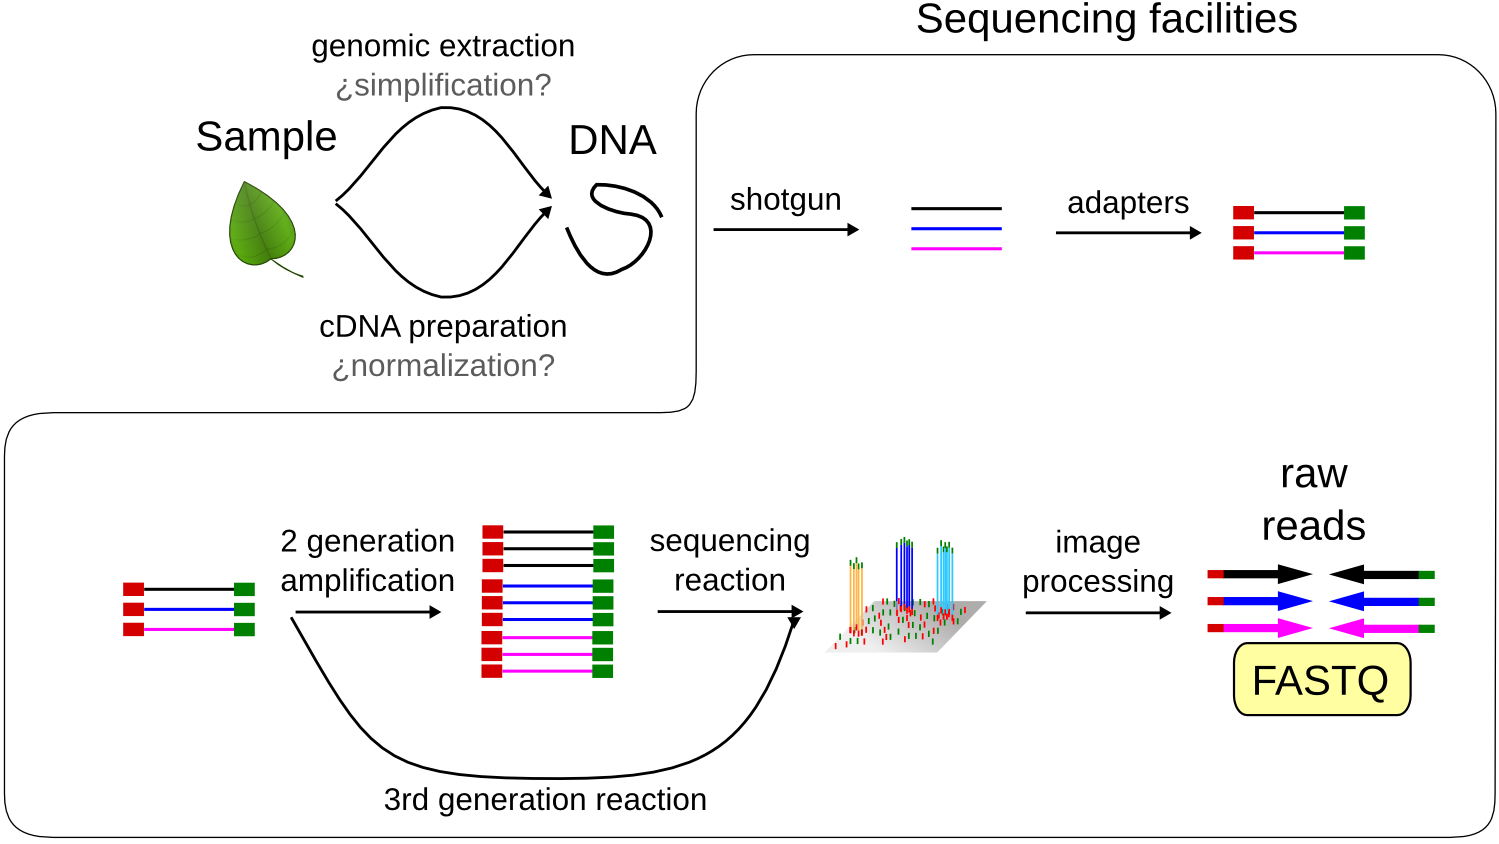
\includegraphics[width=\textwidth]{c2.genomics/workflow.ngs.01.png}
  \end{figure}
\end{frame}

\begin{frame}
  \frametitle{基因组学 | 数据分析 | 流程 | 概述 | 总览}
  \begin{figure}
    \centering
    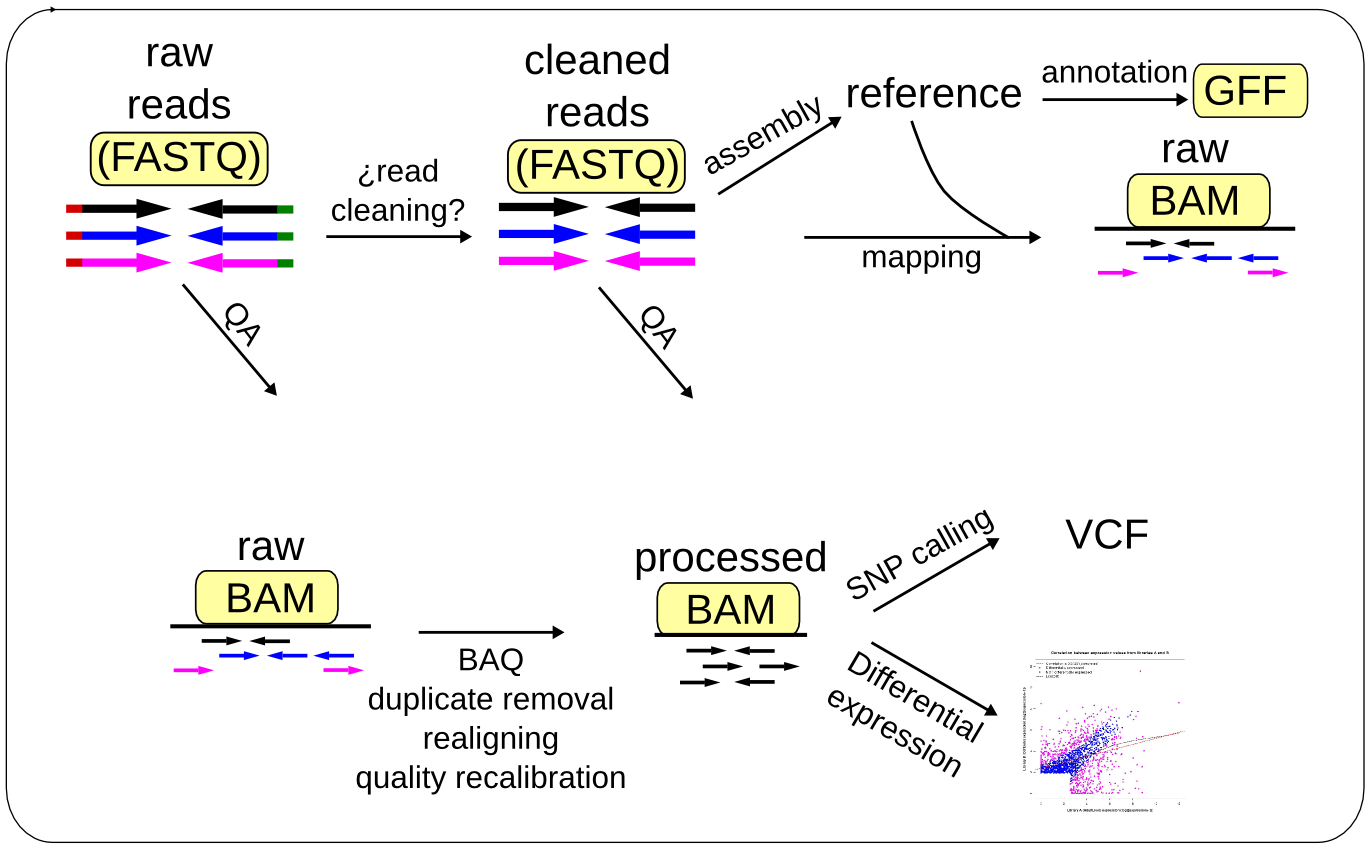
\includegraphics[width=\textwidth]{c2.genomics/workflow.ngs.02.png}
  \end{figure}
\end{frame}

\begin{frame}
  \frametitle{基因组学 | 数据分析 | 流程 | 概述 | \textcolor{red}{Seqs}}
  \begin{figure}
    \centering
    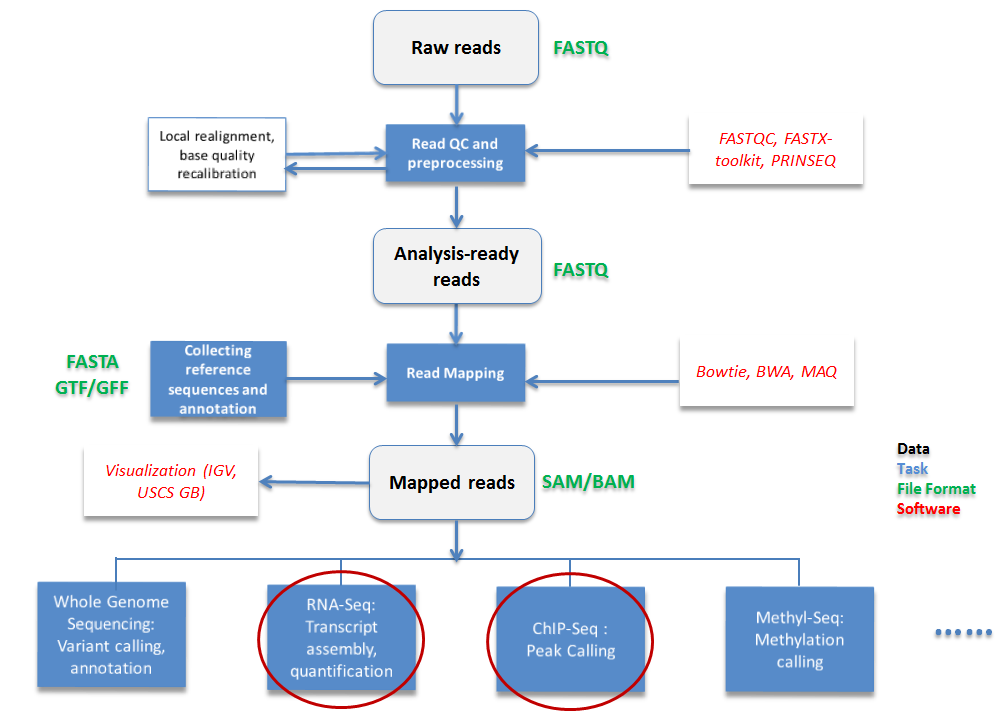
\includegraphics[width=0.9\textwidth]{c2.genomics/workflow.ngs.03.png}
  \end{figure}
\end{frame}

\begin{frame}
  \frametitle{基因组学 | 数据分析 | 流程 | 概述 | Seqs}
  \begin{figure}
    \centering
    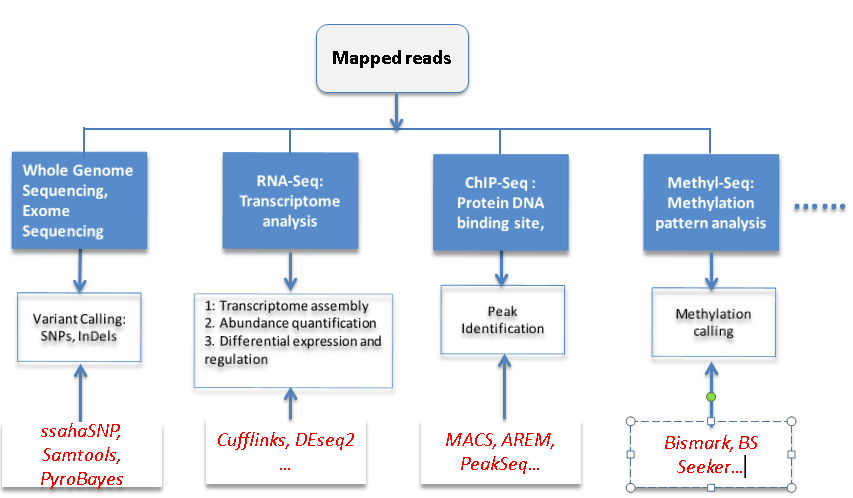
\includegraphics[width=\textwidth]{c2.genomics/workflow.ngs.04.png}
  \end{figure}
\end{frame}

\begin{frame}
  \frametitle{基因组学 | 数据分析 | 流程 | 概述 | 总览}
  \begin{figure}
    \centering
    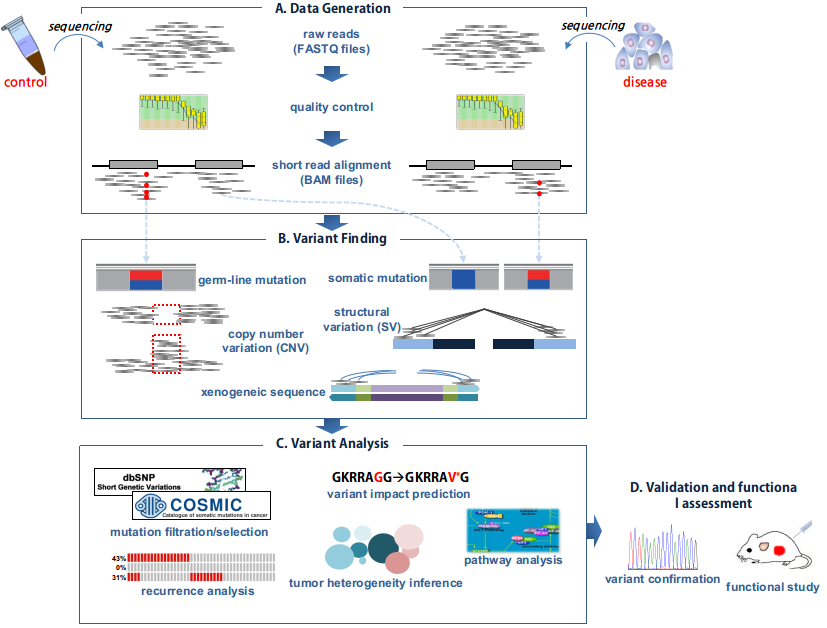
\includegraphics[width=0.85\textwidth]{c2.genomics/workflow.ngs.10.png}
  \end{figure}
\end{frame}

\begin{frame}
  \frametitle{基因组学 | 数据分析 | 流程 | 概述 | \textcolor{red}{Exome}}
  \begin{figure}
    \centering
    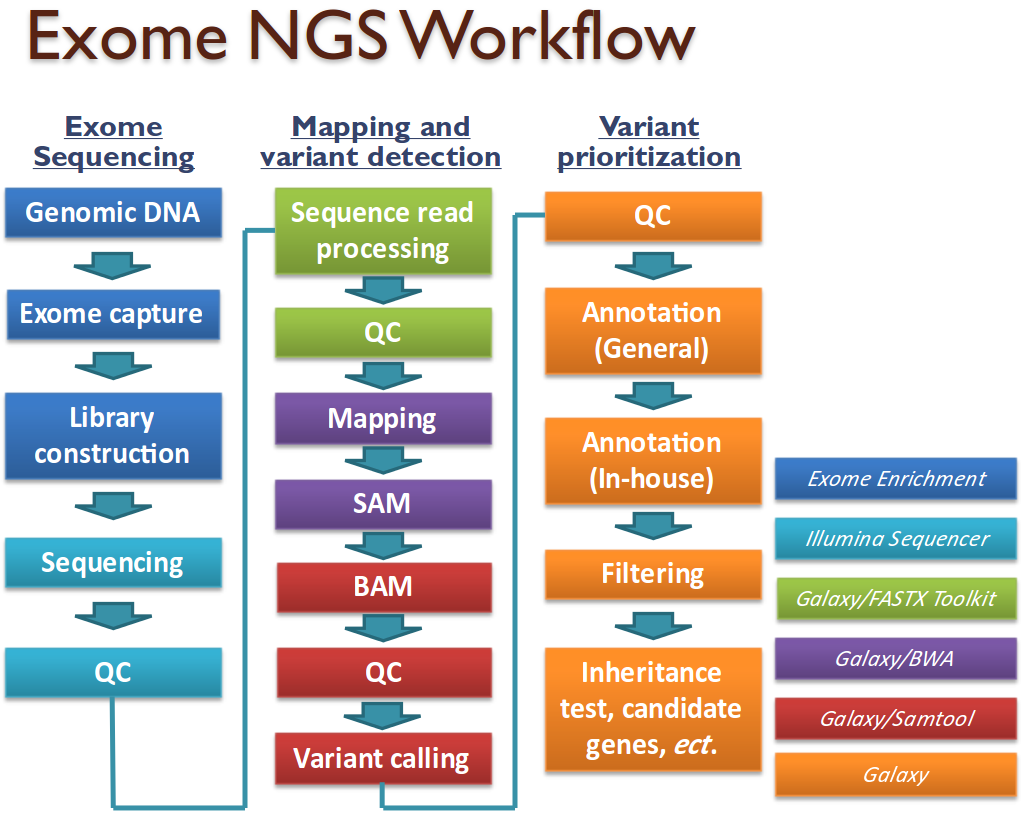
\includegraphics[width=0.9\textwidth]{c2.genomics/workflow.exome.03.png}
  \end{figure}
\end{frame}

\begin{frame}
  \frametitle{基因组学 | 数据分析 | 流程 | 概述 | \textcolor{red}{Exome}}
  \begin{figure}
    \centering
    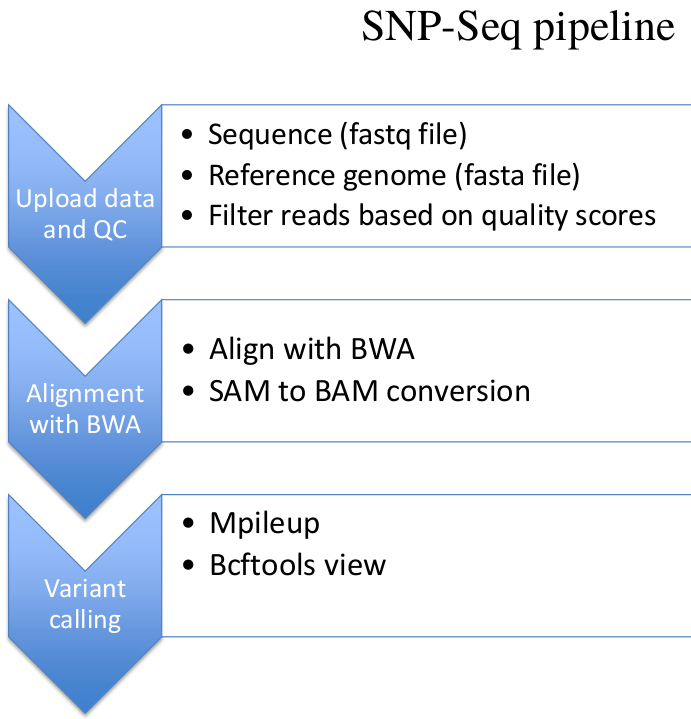
\includegraphics[width=0.6\textwidth]{c2.genomics/workflow.exome.05.png}
  \end{figure}
\end{frame}

\begin{frame}
  \frametitle{基因组学 | 数据分析 | 流程 | 质控(Quality Control)}
  \begin{figure}
    \centering
    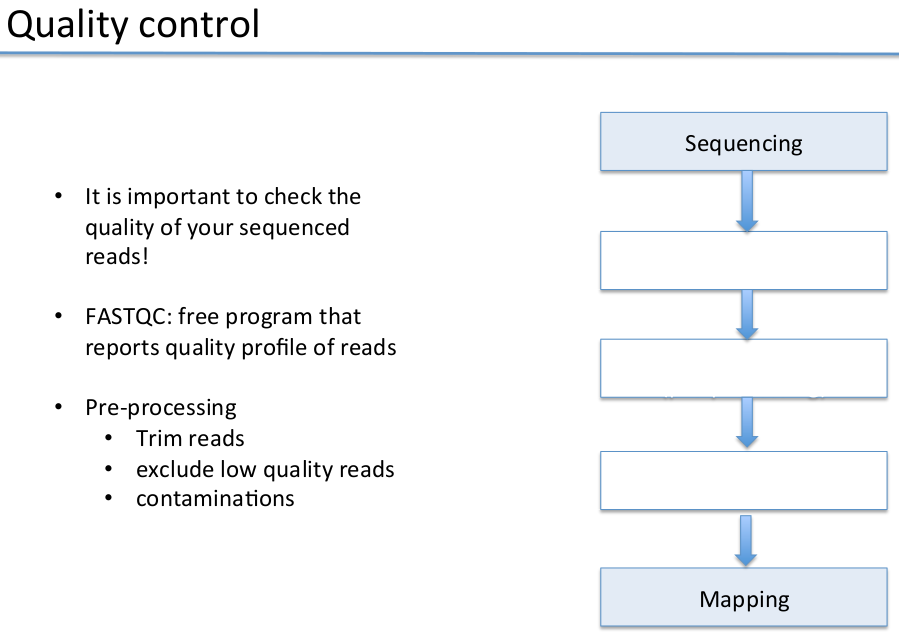
\includegraphics[width=0.9\textwidth]{c2.genomics/qc.pre.01.png}
  \end{figure}
\end{frame}

\begin{frame}
  \frametitle{基因组学 | 数据分析 | 流程 | 质控}
  \begin{figure}
    \centering
    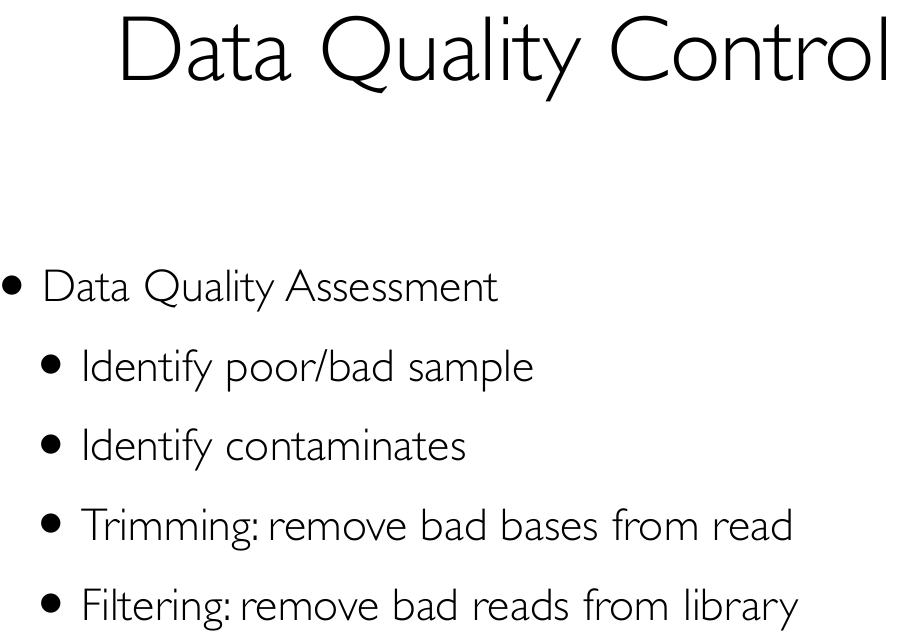
\includegraphics[width=0.9\textwidth]{c2.genomics/qc.pre.02.png}
  \end{figure}
\end{frame}

\begin{frame}
  \frametitle{基因组学 | 数据分析 | 流程 | 质控}
  \begin{figure}
    \centering
    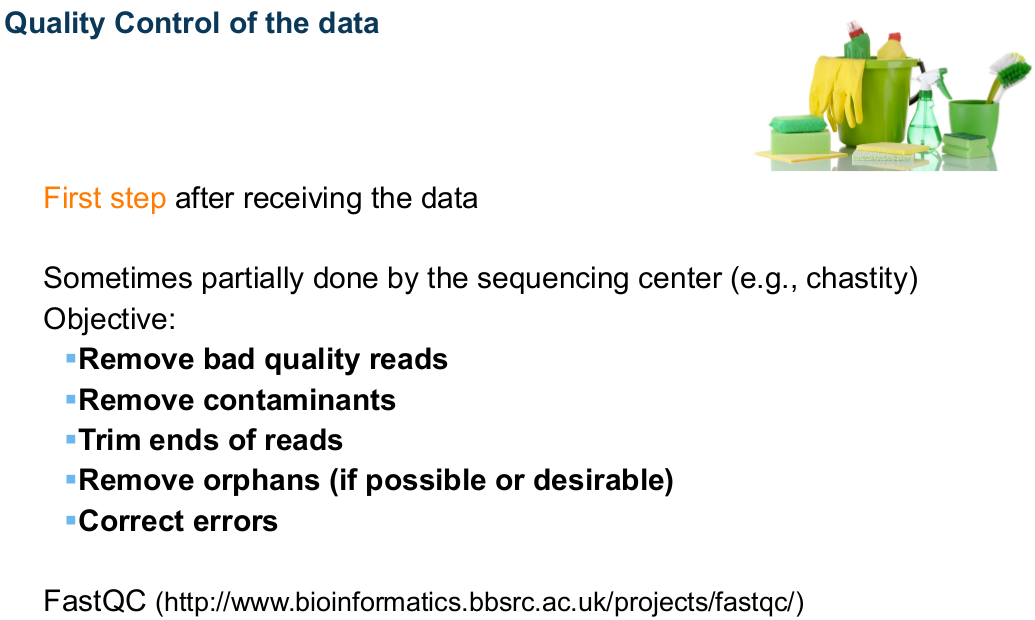
\includegraphics[width=0.9\textwidth]{c2.genomics/qc.pre.04.png}
  \end{figure}
\end{frame}

\begin{frame}
  \frametitle{基因组学 | 数据分析 | 流程 | 质控}
  \begin{figure}
    \centering
    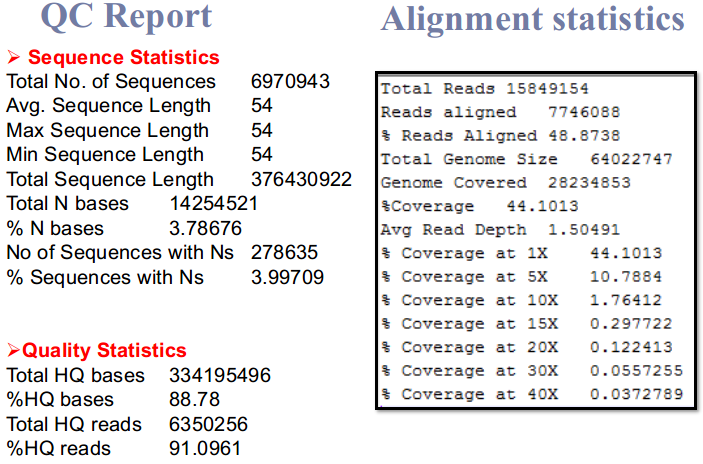
\includegraphics[width=0.9\textwidth]{c2.genomics/qc.report.01.png}
  \end{figure}
\end{frame}

\begin{frame}
  \frametitle{基因组学 | 数据分析 | 流程 | 质控 | 工具}
  \begin{figure}
    \centering
    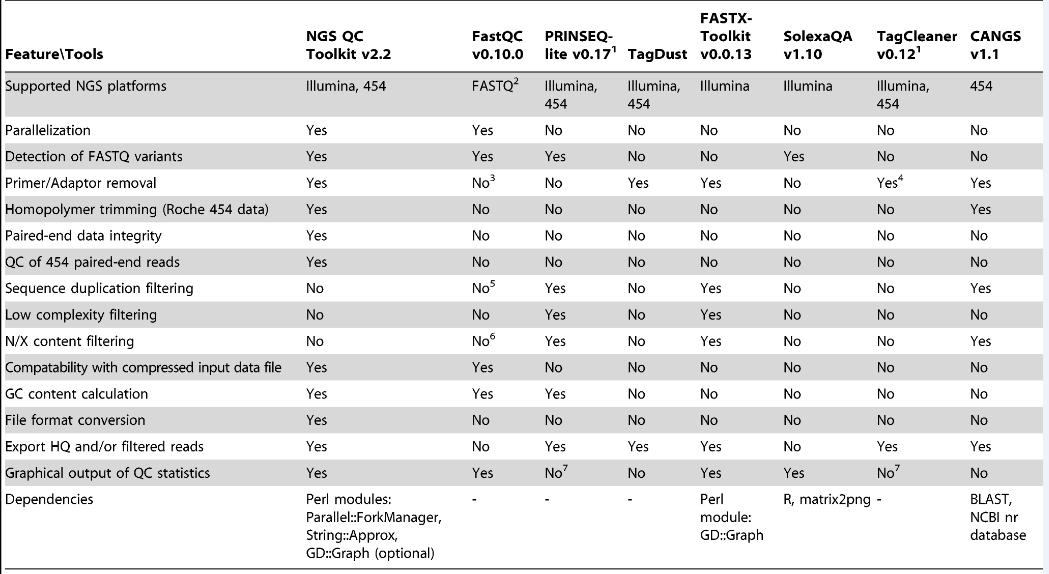
\includegraphics[width=\textwidth]{c2.genomics/qc.tool.01.png}
  \end{figure}
\end{frame}

\begin{frame}
  \frametitle{基因组学 | 数据分析 | 流程 | 质控 | \textcolor{red}{工具}}
  \begin{block}{FastQC}
    A quality control tool for high throughput sequence data.
  \end{block}
  \pause
  \begin{block}{NGS QC Toolkit}
    A toolkit for the quality control (QC) of next generation sequencing (NGS) data.
  \end{block}
  \pause
  \begin{block}{Others}
    \begin{itemize}
      \item SolexaQA: calculates sequence quality statistics and creates visual representations of data quality for second-generation sequencing data.
      \item ...
    \end{itemize}
  \end{block}
\end{frame}

\begin{frame}
  \frametitle{基因组学 | 数据分析 | 流程 | 质控 | FastQC}
  \begin{figure}
    \centering
    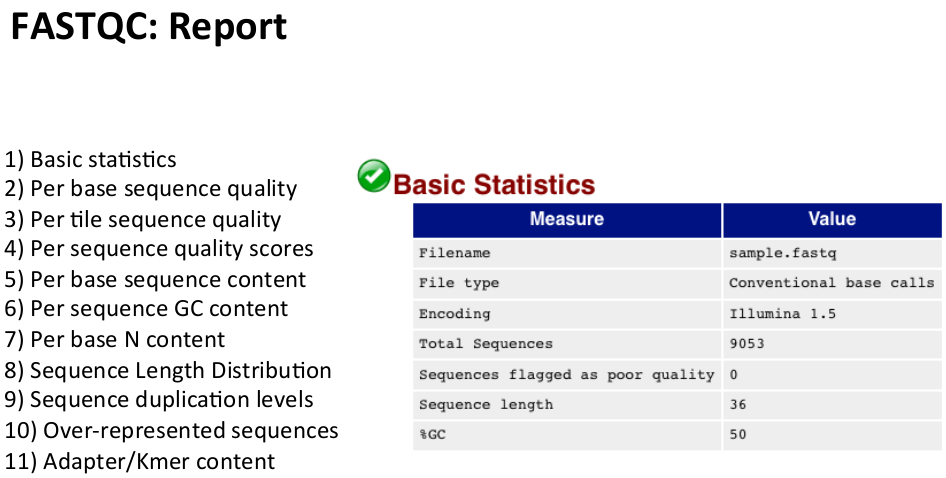
\includegraphics[width=0.9\textwidth]{c2.genomics/qc.fastqc.00.png}
  \end{figure}
\end{frame}

\begin{frame}
  \frametitle{基因组学 | 数据分析 | 流程 | 质控 | FastQC}
  \begin{figure}
    \centering
    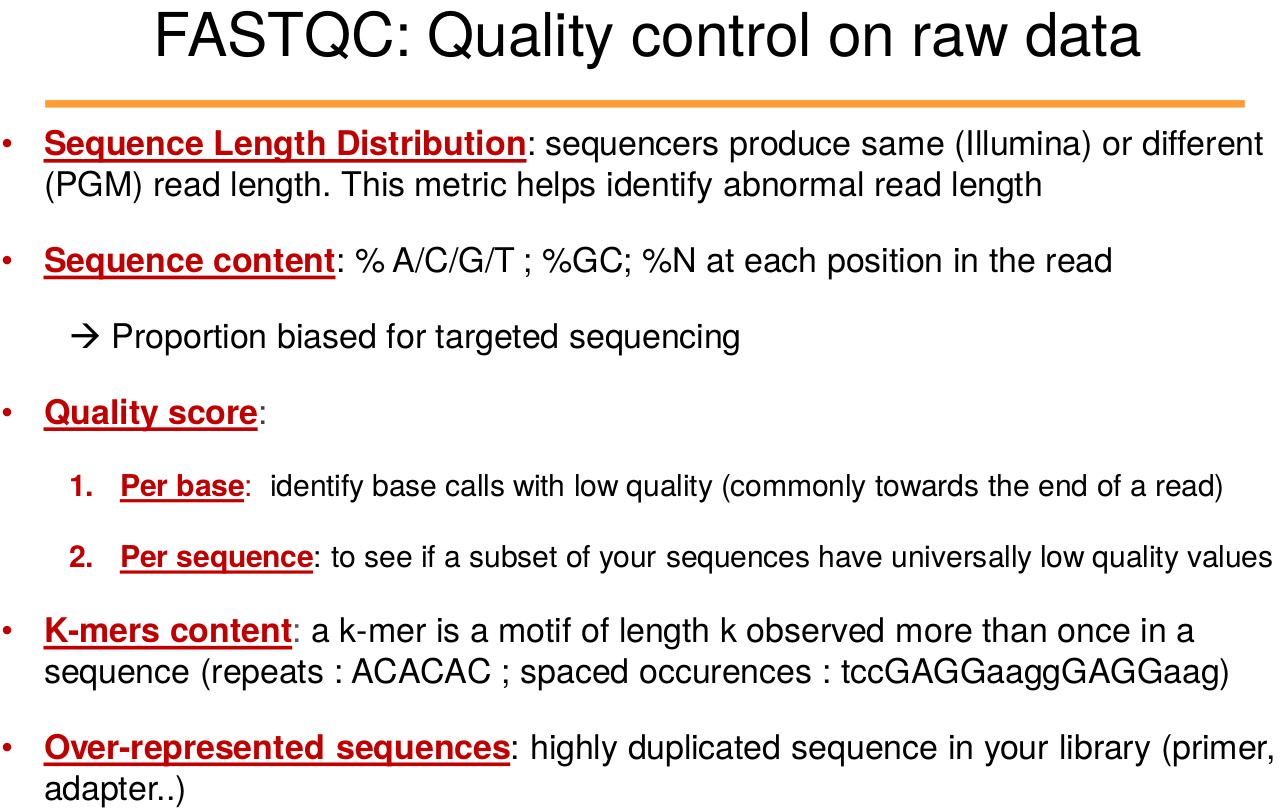
\includegraphics[width=0.9\textwidth]{c2.genomics/qc.fastqc.03.png}
  \end{figure}
\end{frame}

\begin{frame}
  \frametitle{基因组学 | 数据分析 | 流程 | 质控 | FastQC}
  \begin{figure}
    \centering
    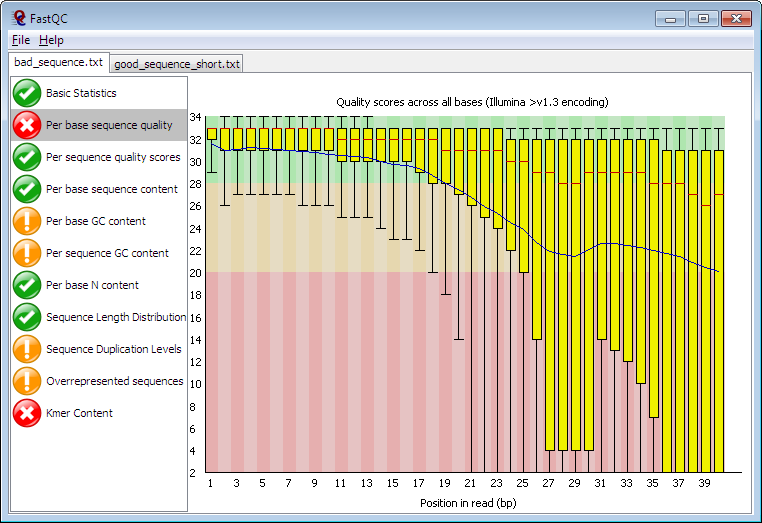
\includegraphics[width=0.9\textwidth]{c2.genomics/qc.fastqc.01.png}
  \end{figure}
\end{frame}

\begin{frame}
  \frametitle{基因组学 | 数据分析 | 流程 | 质控 | FastQC}
  \begin{figure}
    \centering
    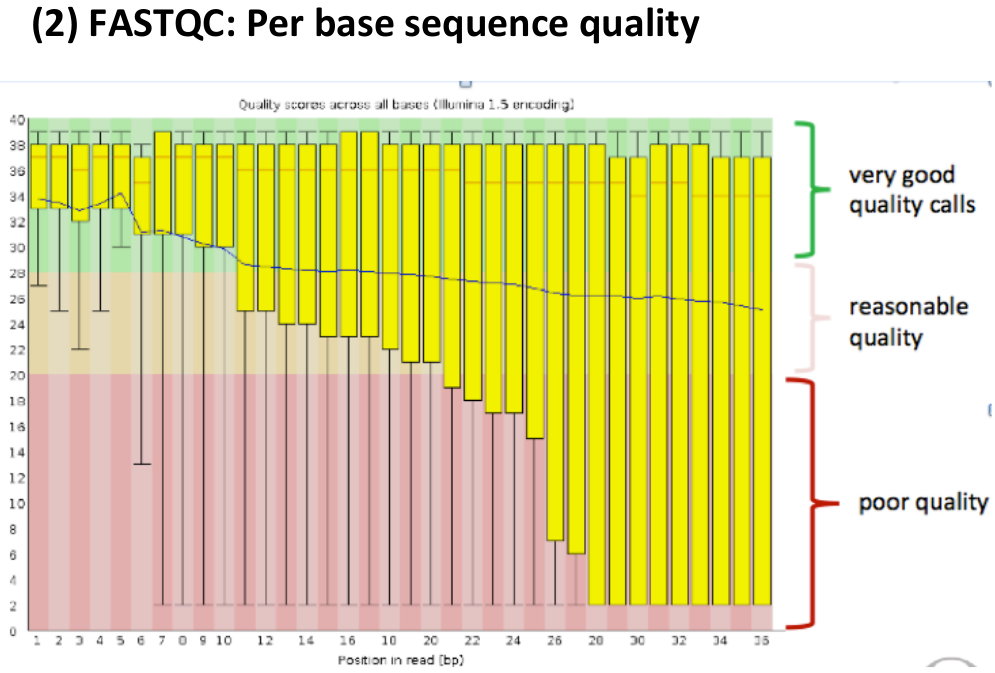
\includegraphics[width=0.9\textwidth]{c2.genomics/qc.fastqc.02.png}
  \end{figure}
\end{frame}

\begin{frame}
  \frametitle{基因组学 | 数据分析 | 流程 | 质控 | FastQC}
  \begin{figure}
    \centering
    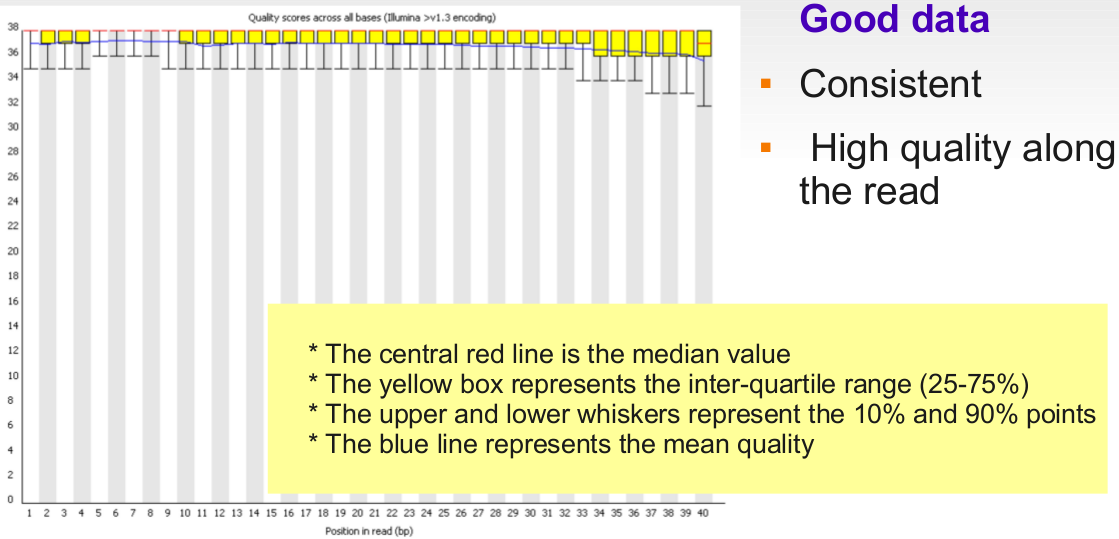
\includegraphics[width=\textwidth]{c2.genomics/qc.fastqc.10.png}
  \end{figure}
\end{frame}

\begin{frame}
  \frametitle{基因组学 | 数据分析 | 流程 | 质控 | FastQC}
  \begin{figure}
    \centering
    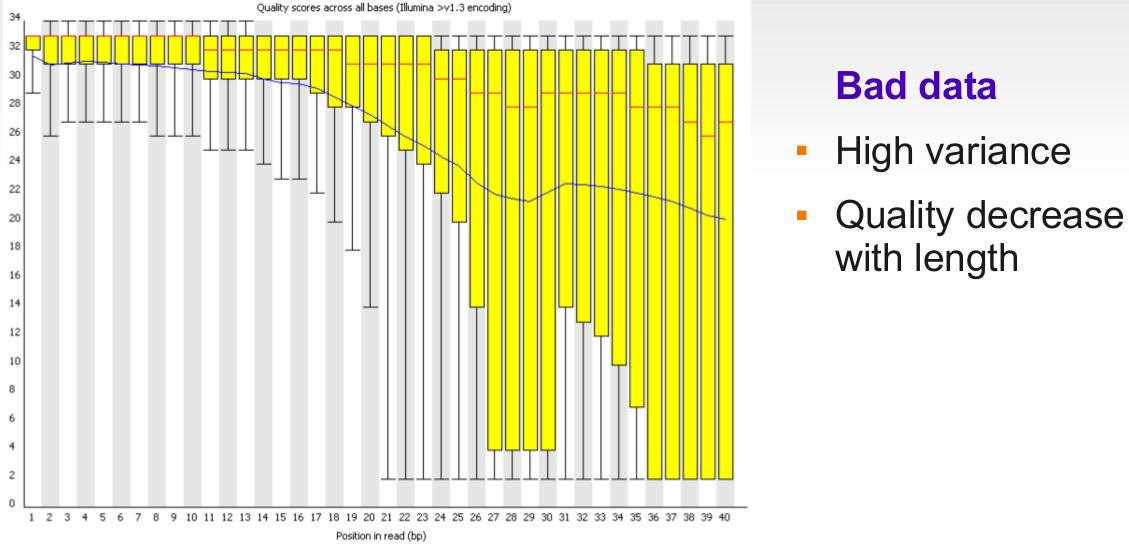
\includegraphics[width=\textwidth]{c2.genomics/qc.fastqc.11.png}
  \end{figure}
\end{frame}

\begin{frame}
  \frametitle{基因组学 | 数据分析 | 流程 | 质控 | FastQC}
  \begin{figure}
    \centering
    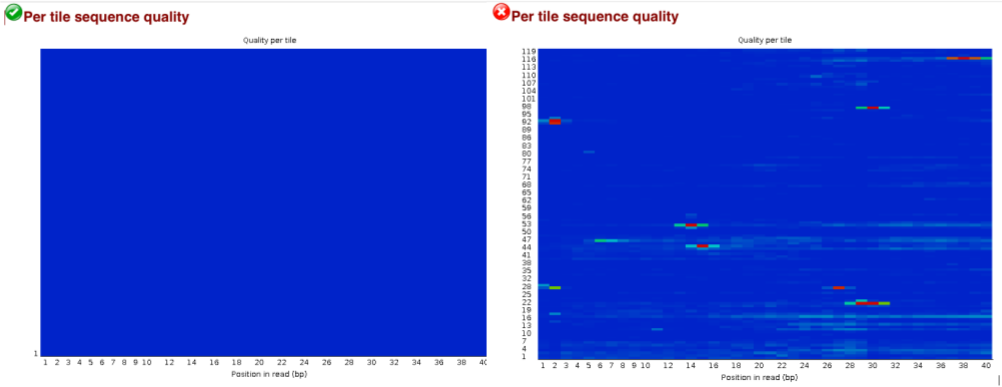
\includegraphics[width=\textwidth]{c2.genomics/qc.fastqc.30.png}
  \end{figure}
\end{frame}

\begin{frame}
  \frametitle{基因组学 | 数据分析 | 流程 | 质控 | FastQC}
  \begin{figure}
    \centering
    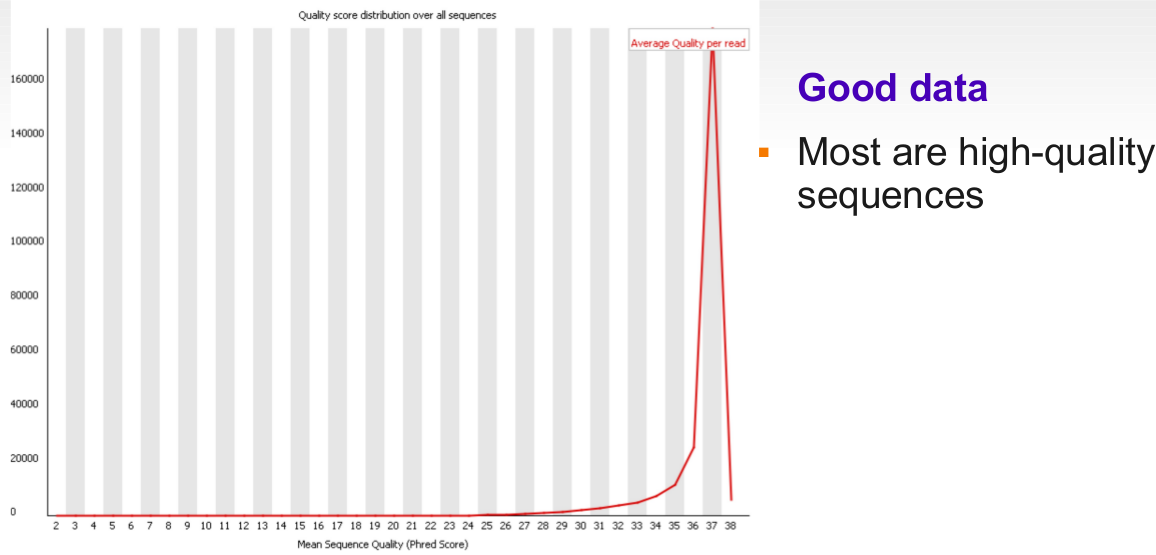
\includegraphics[width=\textwidth]{c2.genomics/qc.fastqc.12.png}
  \end{figure}
\end{frame}

\begin{frame}
  \frametitle{基因组学 | 数据分析 | 流程 | 质控 | FastQC}
  \begin{figure}
    \centering
    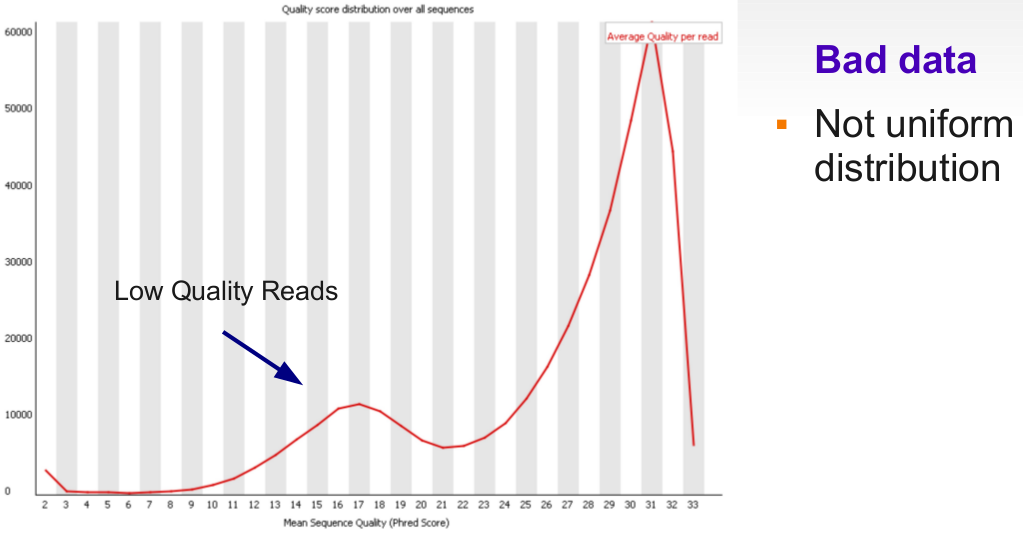
\includegraphics[width=\textwidth]{c2.genomics/qc.fastqc.13.png}
  \end{figure}
\end{frame}

\begin{frame}
  \frametitle{基因组学 | 数据分析 | 流程 | 质控 | FastQC}
  \begin{figure}
    \centering
    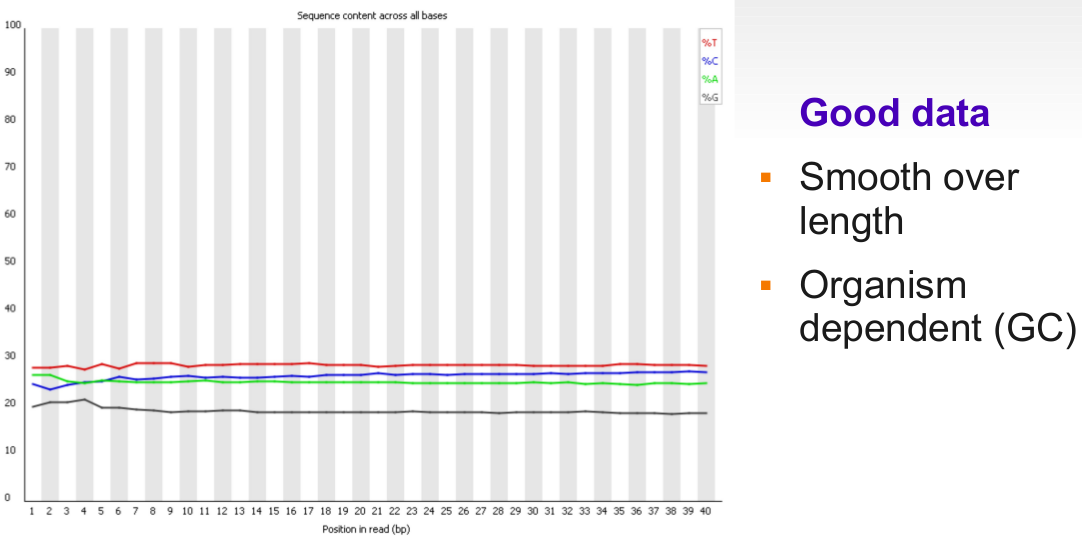
\includegraphics[width=\textwidth]{c2.genomics/qc.fastqc.14.png}
  \end{figure}
\end{frame}

\begin{frame}
  \frametitle{基因组学 | 数据分析 | 流程 | 质控 | FastQC}
  \begin{figure}
    \centering
    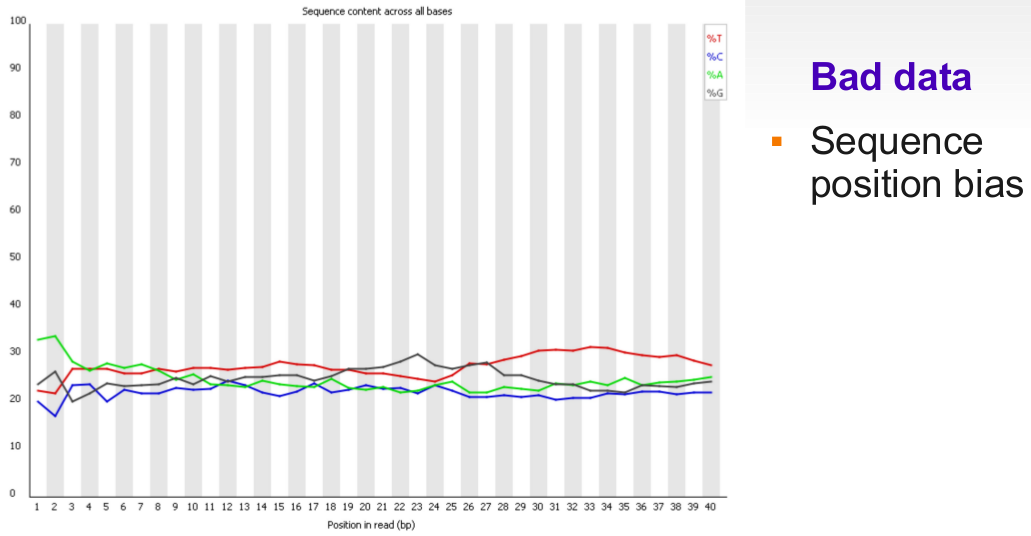
\includegraphics[width=\textwidth]{c2.genomics/qc.fastqc.15.png}
  \end{figure}
\end{frame}

\begin{frame}
  \frametitle{基因组学 | 数据分析 | 流程 | 质控 | FastQC}
  \begin{figure}
    \centering
    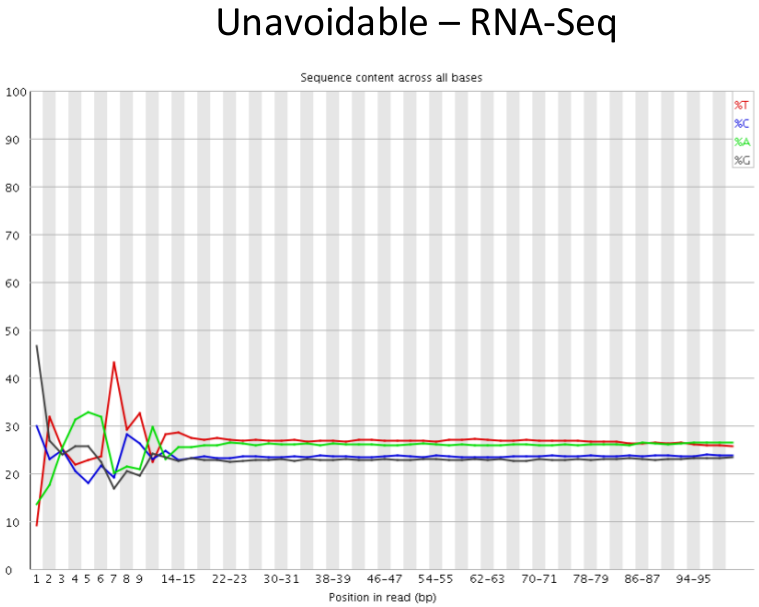
\includegraphics[width=0.9\textwidth]{c2.genomics/qc.fastqc.31.png}
  \end{figure}
\end{frame}

\begin{frame}
  \frametitle{基因组学 | 数据分析 | 流程 | 质控 | FastQC}
  \begin{figure}
    \centering
    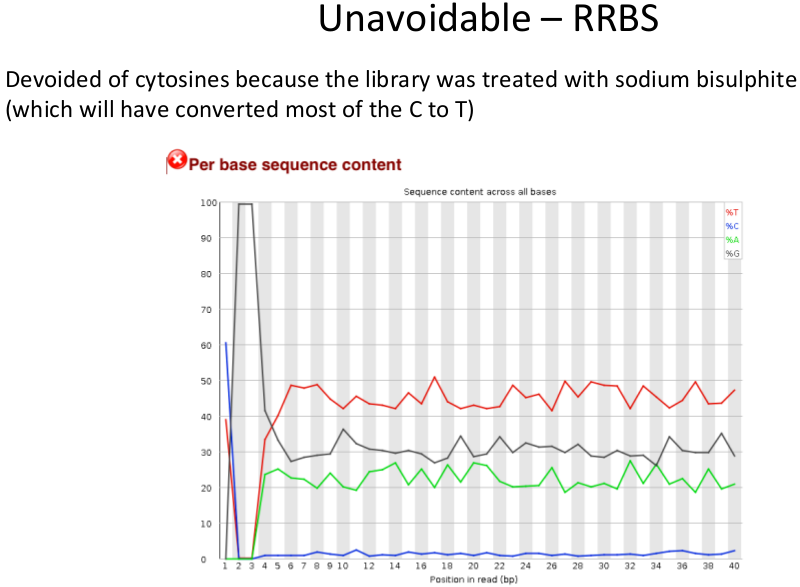
\includegraphics[width=0.9\textwidth]{c2.genomics/qc.fastqc.32.png}
  \end{figure}
\end{frame}

\begin{frame}
  \frametitle{基因组学 | 数据分析 | 流程 | 质控 | FastQC}
  \begin{figure}
    \centering
    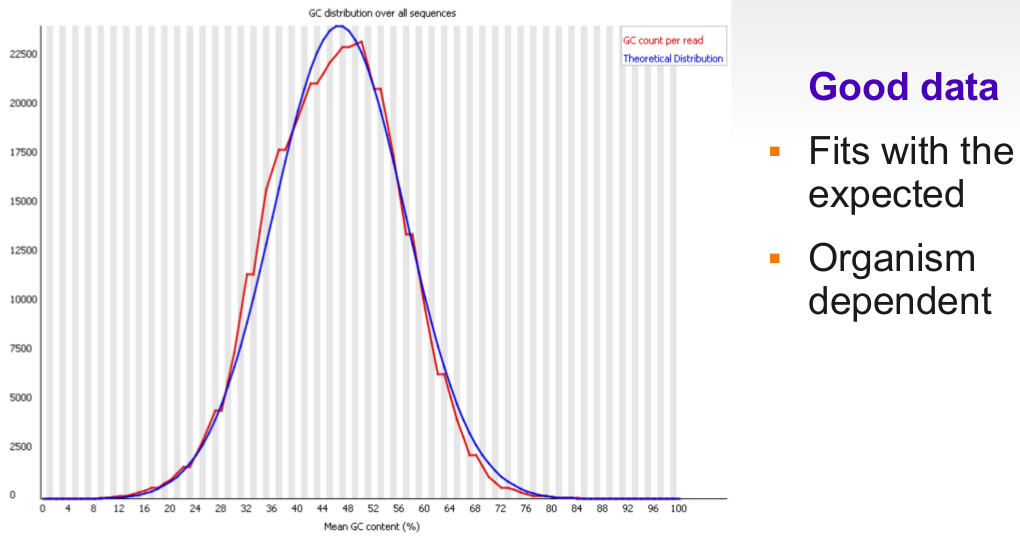
\includegraphics[width=\textwidth]{c2.genomics/qc.fastqc.16.png}
  \end{figure}
\end{frame}

\begin{frame}
  \frametitle{基因组学 | 数据分析 | 流程 | 质控 | FastQC}
  \begin{figure}
    \centering
    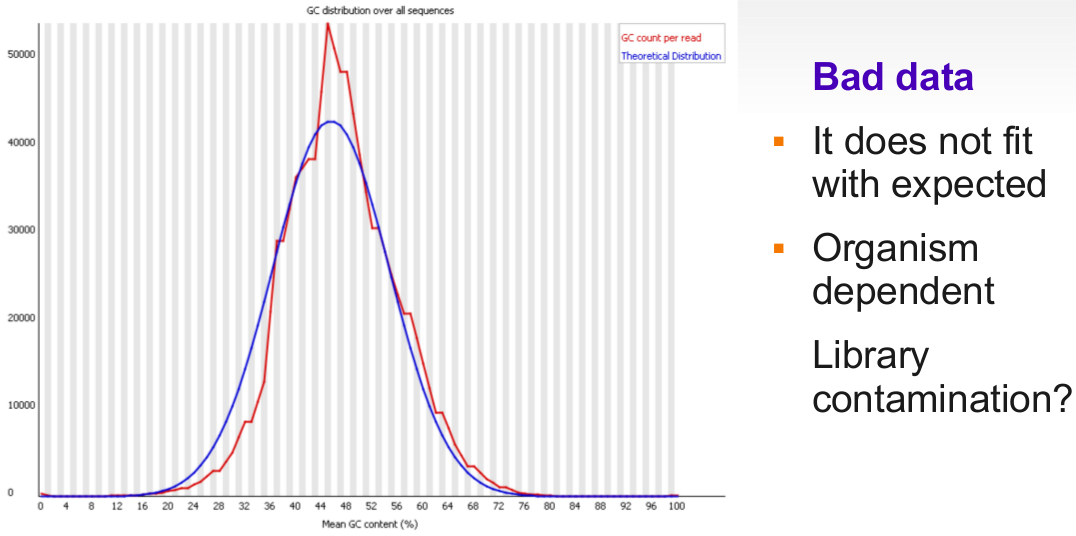
\includegraphics[width=\textwidth]{c2.genomics/qc.fastqc.17.png}
  \end{figure}
\end{frame}

\begin{frame}
  \frametitle{基因组学 | 数据分析 | 流程 | 质控 | FastQC}
  \begin{figure}
    \centering
    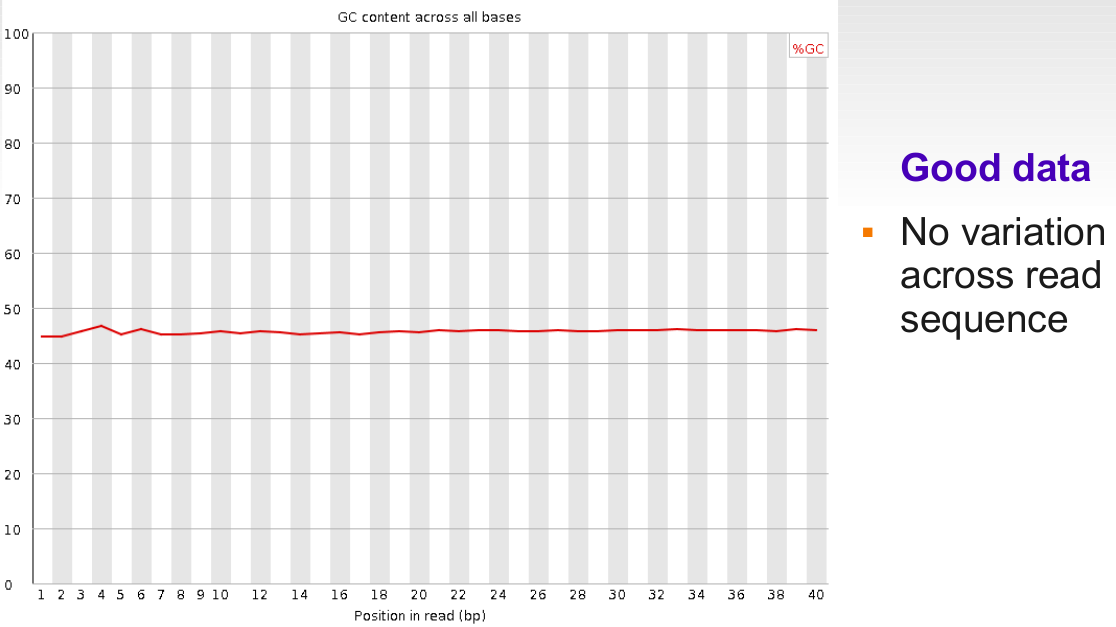
\includegraphics[width=\textwidth]{c2.genomics/qc.fastqc.18.png}
  \end{figure}
\end{frame}

\begin{frame}
  \frametitle{基因组学 | 数据分析 | 流程 | 质控 | FastQC}
  \begin{figure}
    \centering
    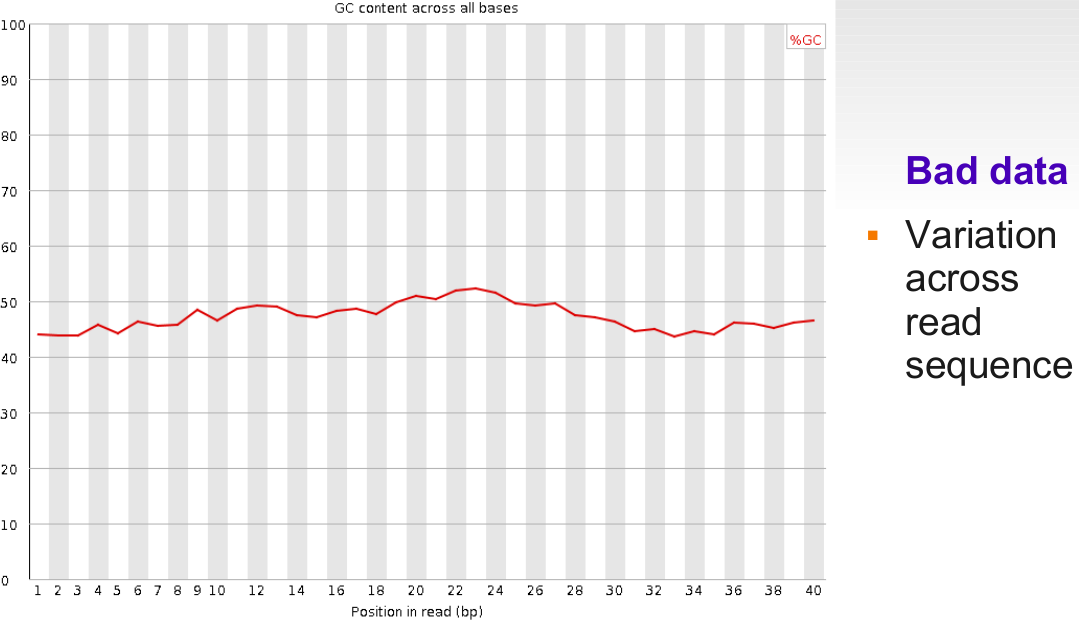
\includegraphics[width=\textwidth]{c2.genomics/qc.fastqc.19.png}
  \end{figure}
\end{frame}

\begin{frame}
  \frametitle{基因组学 | 数据分析 | 流程 | 质控 | FastQC}
  \begin{figure}
    \centering
    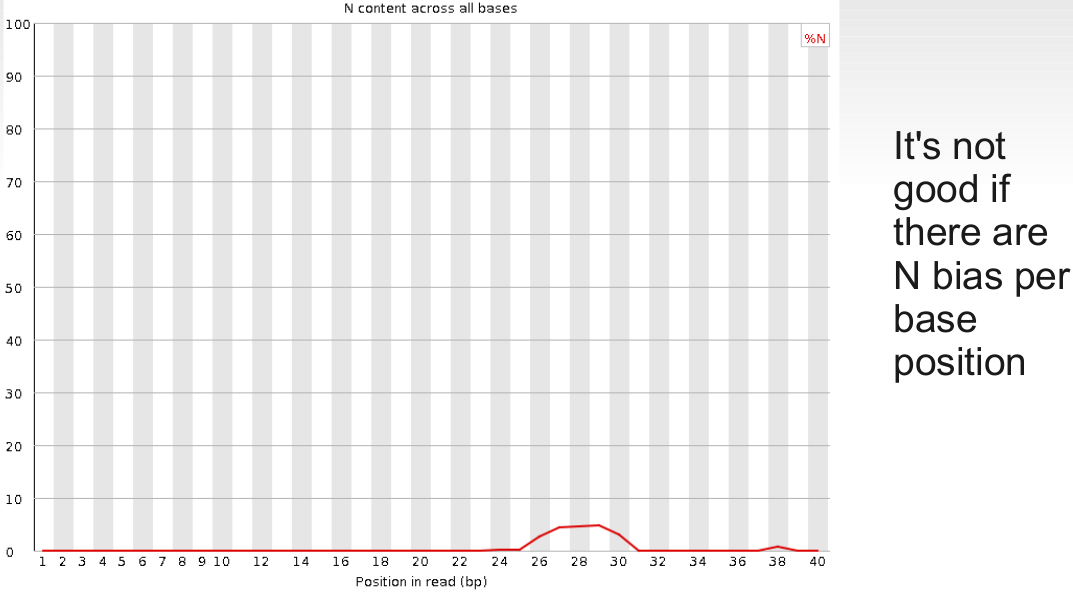
\includegraphics[width=\textwidth]{c2.genomics/qc.fastqc.20.png}
  \end{figure}
\end{frame}

\begin{frame}
  \frametitle{基因组学 | 数据分析 | 流程 | 质控 | FastQC}
  \begin{figure}
    \centering
    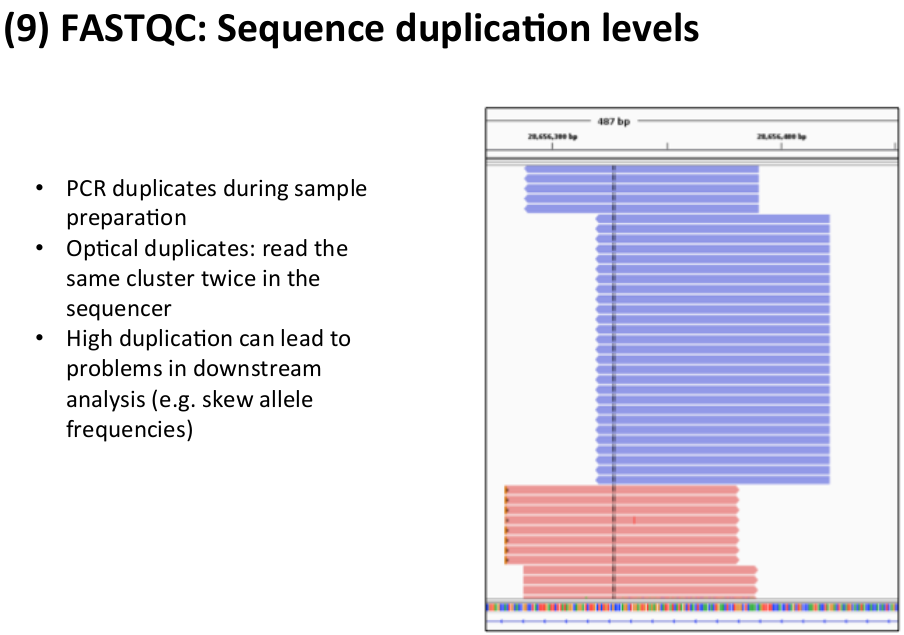
\includegraphics[width=0.9\textwidth]{c2.genomics/qc.fastqc.33.png}
  \end{figure}
\end{frame}

\begin{frame}
  \frametitle{基因组学 | 数据分析 | 流程 | 质控 | FastQC}
  \begin{figure}
    \centering
    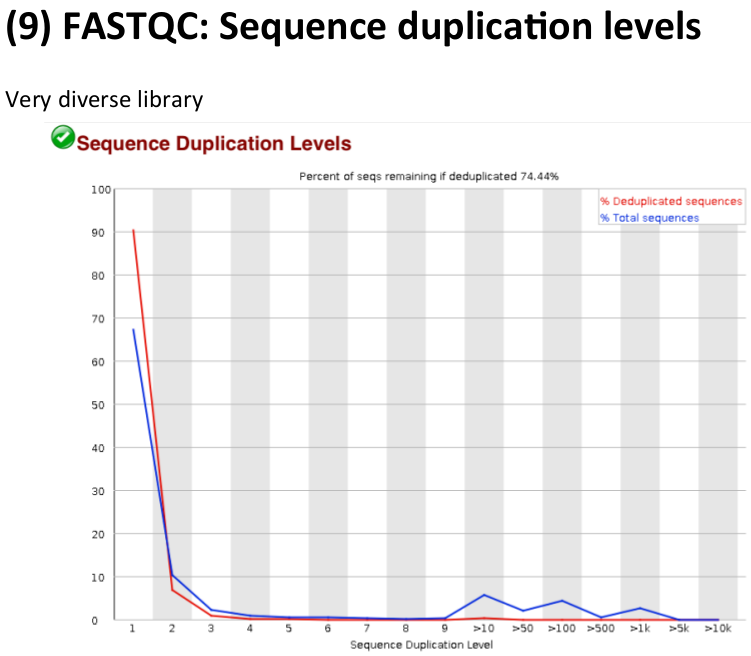
\includegraphics[width=0.7\textwidth]{c2.genomics/qc.fastqc.34.png}
  \end{figure}
\end{frame}

\begin{frame}
  \frametitle{基因组学 | 数据分析 | 流程 | 质控 | FastQC}
  \begin{figure}
    \centering
    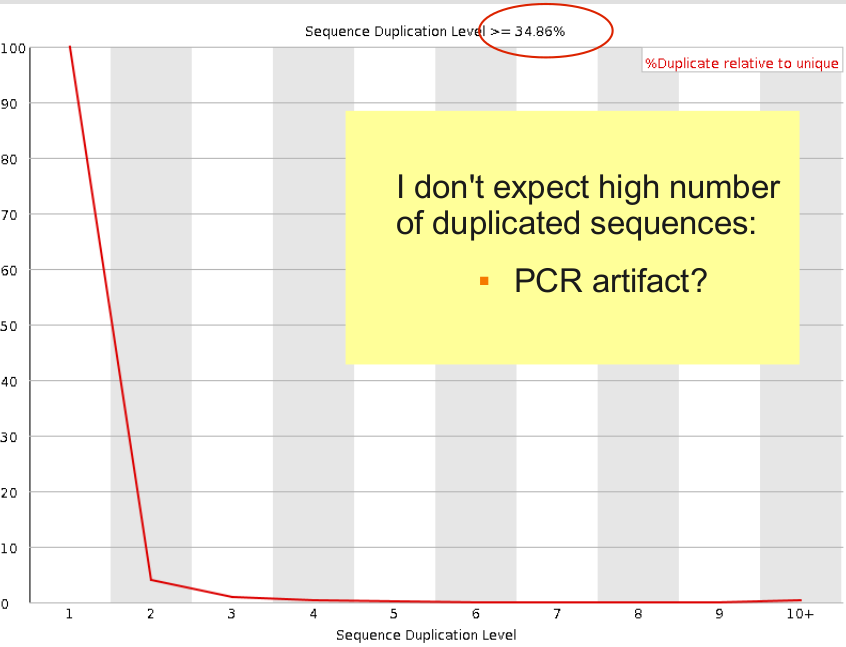
\includegraphics[width=0.85\textwidth]{c2.genomics/qc.fastqc.21.png}
  \end{figure}
\end{frame}

\begin{frame}
  \frametitle{基因组学 | 数据分析 | 流程 | 质控 | FastQC}
  \begin{figure}
    \centering
    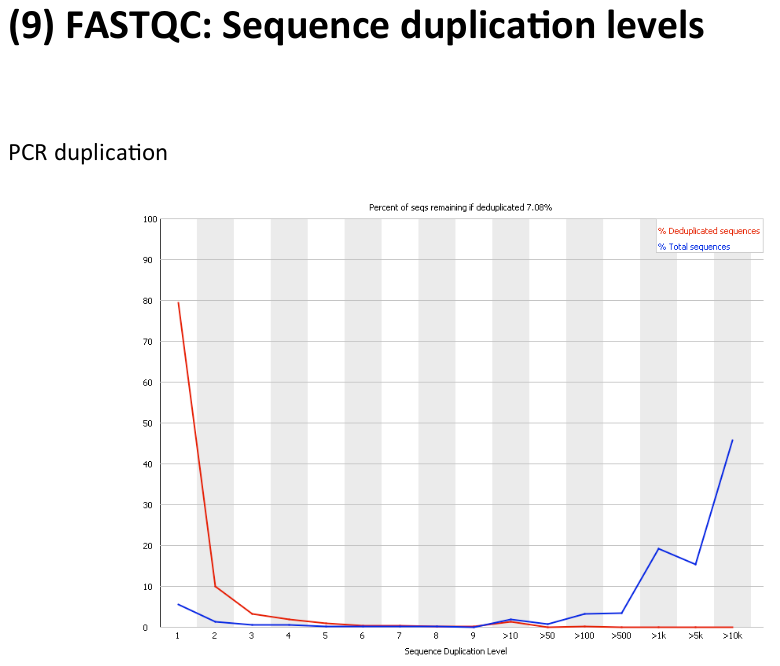
\includegraphics[width=0.7\textwidth]{c2.genomics/qc.fastqc.36.png}
  \end{figure}
\end{frame}

\begin{frame}
  \frametitle{基因组学 | 数据分析 | 流程 | 质控 | FastQC}
  \begin{figure}
    \centering
    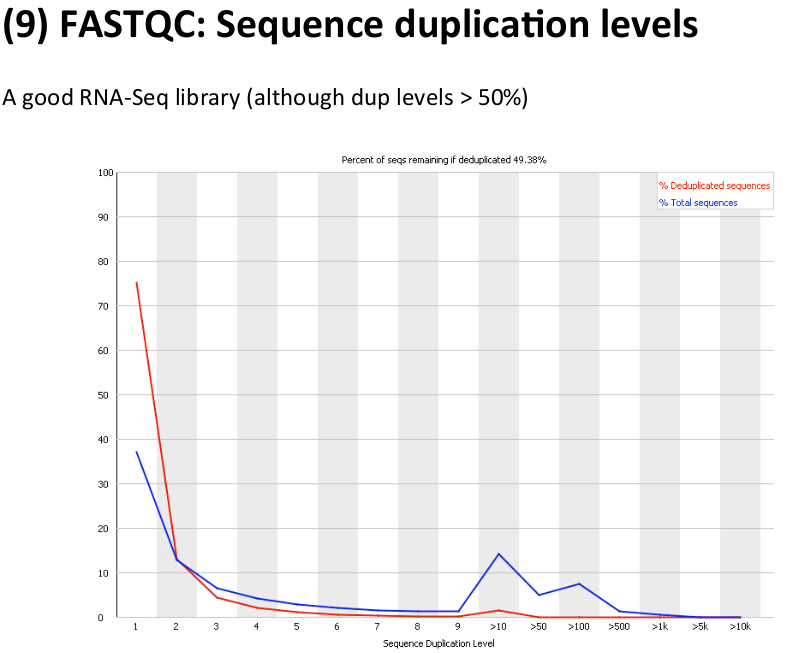
\includegraphics[width=0.8\textwidth]{c2.genomics/qc.fastqc.35.png}
  \end{figure}
\end{frame}

\begin{frame}
  \frametitle{基因组学 | 数据分析 | 流程 | 质控 | FastQC}
  \begin{figure}
    \centering
    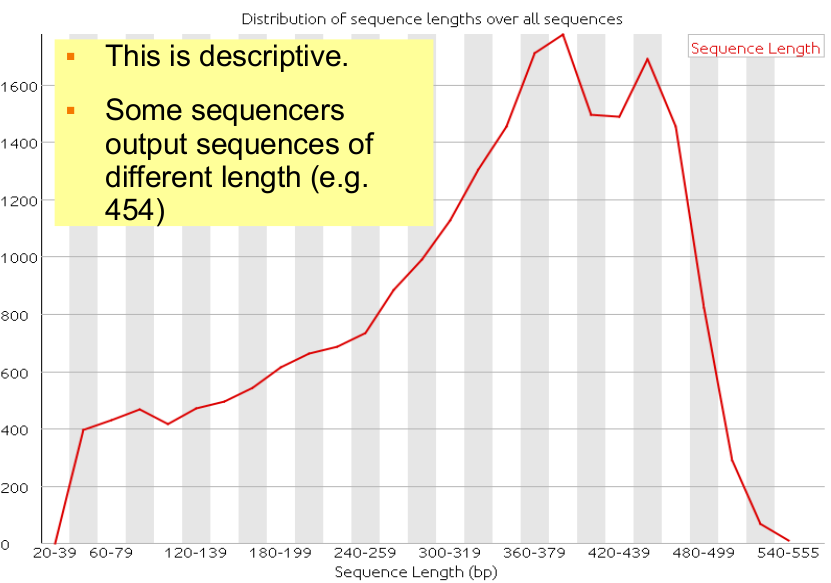
\includegraphics[width=0.9\textwidth]{c2.genomics/qc.fastqc.22.png}
  \end{figure}
\end{frame}

\begin{frame}
  \frametitle{基因组学 | 数据分析 | 流程 | 质控 | FastQC}
  \begin{figure}
    \centering
    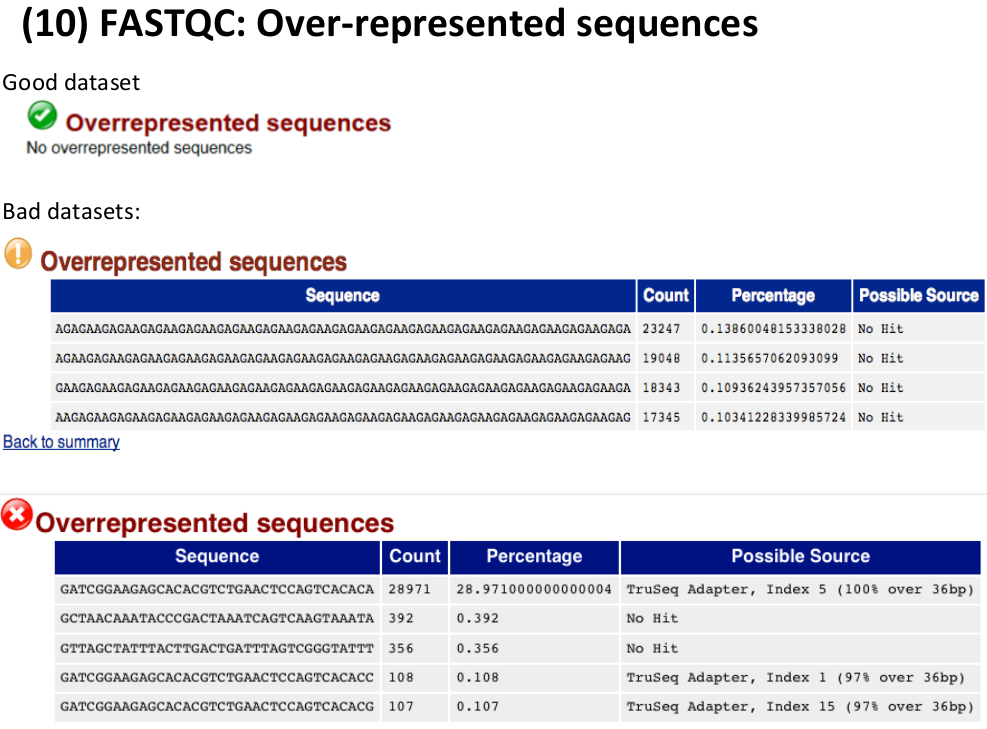
\includegraphics[width=0.9\textwidth]{c2.genomics/qc.fastqc.37.png}
  \end{figure}
\end{frame}

\begin{frame}
  \frametitle{基因组学 | 数据分析 | 流程 | 质控 | FastQC}
  \begin{figure}
    \centering
    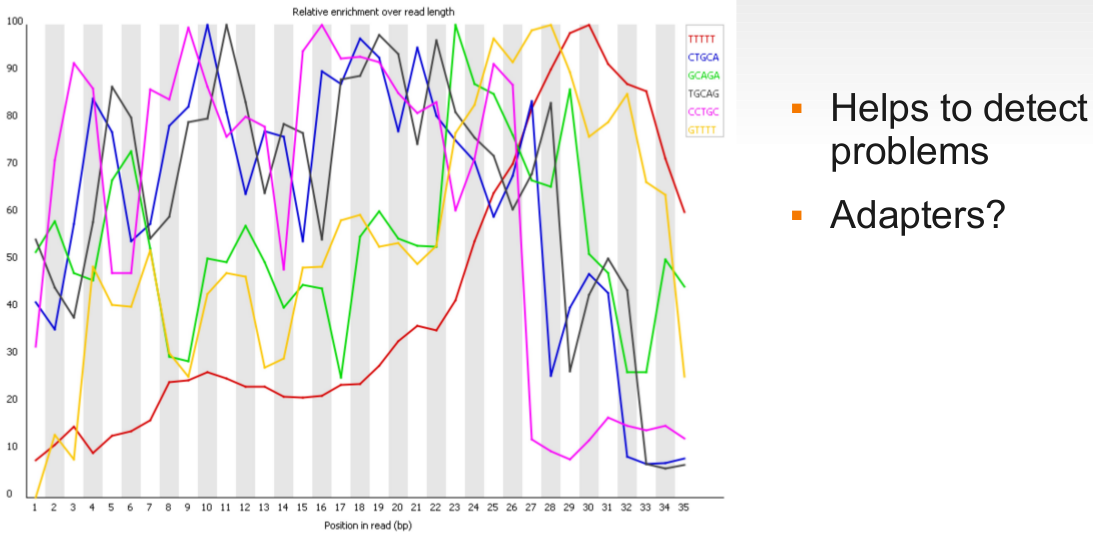
\includegraphics[width=\textwidth]{c2.genomics/qc.fastqc.23.png}
  \end{figure}
\end{frame}

\begin{frame}
  \frametitle{基因组学 | 数据分析 | 流程 | 质控 | FastQC}
  \begin{figure}
    \centering
    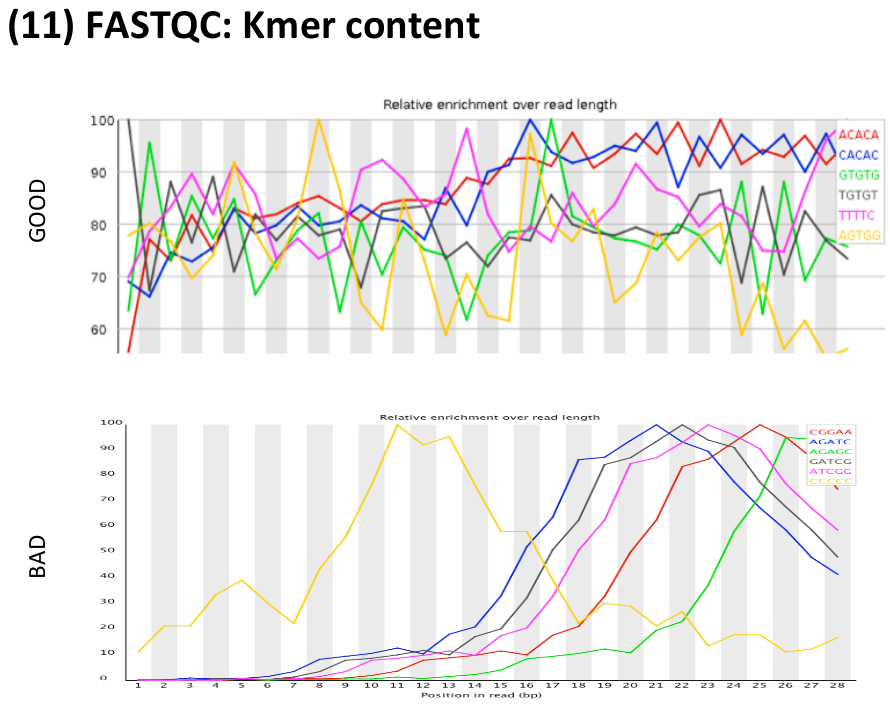
\includegraphics[width=0.8\textwidth]{c2.genomics/qc.fastqc.24.png}
  \end{figure}
\end{frame}

\begin{frame}
  \frametitle{基因组学 | 数据分析 | 流程 | 质控 | FastQC}
  \begin{figure}
    \centering
    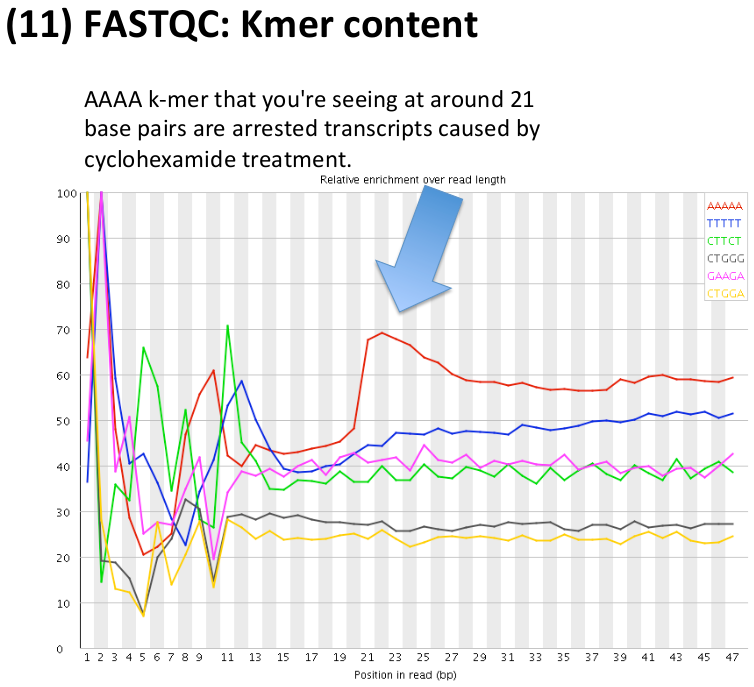
\includegraphics[width=0.7\textwidth]{c2.genomics/qc.fastqc.25.png}
  \end{figure}
\end{frame}

\begin{frame}
  \frametitle{基因组学 | 数据分析 | 流程 | 质控 | FastQC}
  \begin{figure}
    \centering
    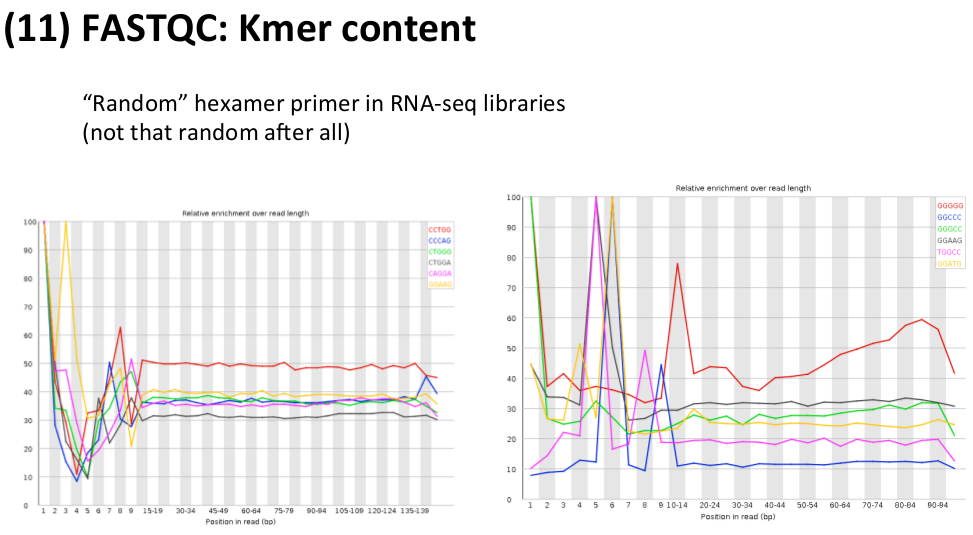
\includegraphics[width=\textwidth]{c2.genomics/qc.fastqc.26.png}
  \end{figure}
\end{frame}

\begin{frame}
  \frametitle{基因组学 | 数据分析 | 流程 | 质控 | NGS QC Toolkit}
  \begin{figure}
    \centering
    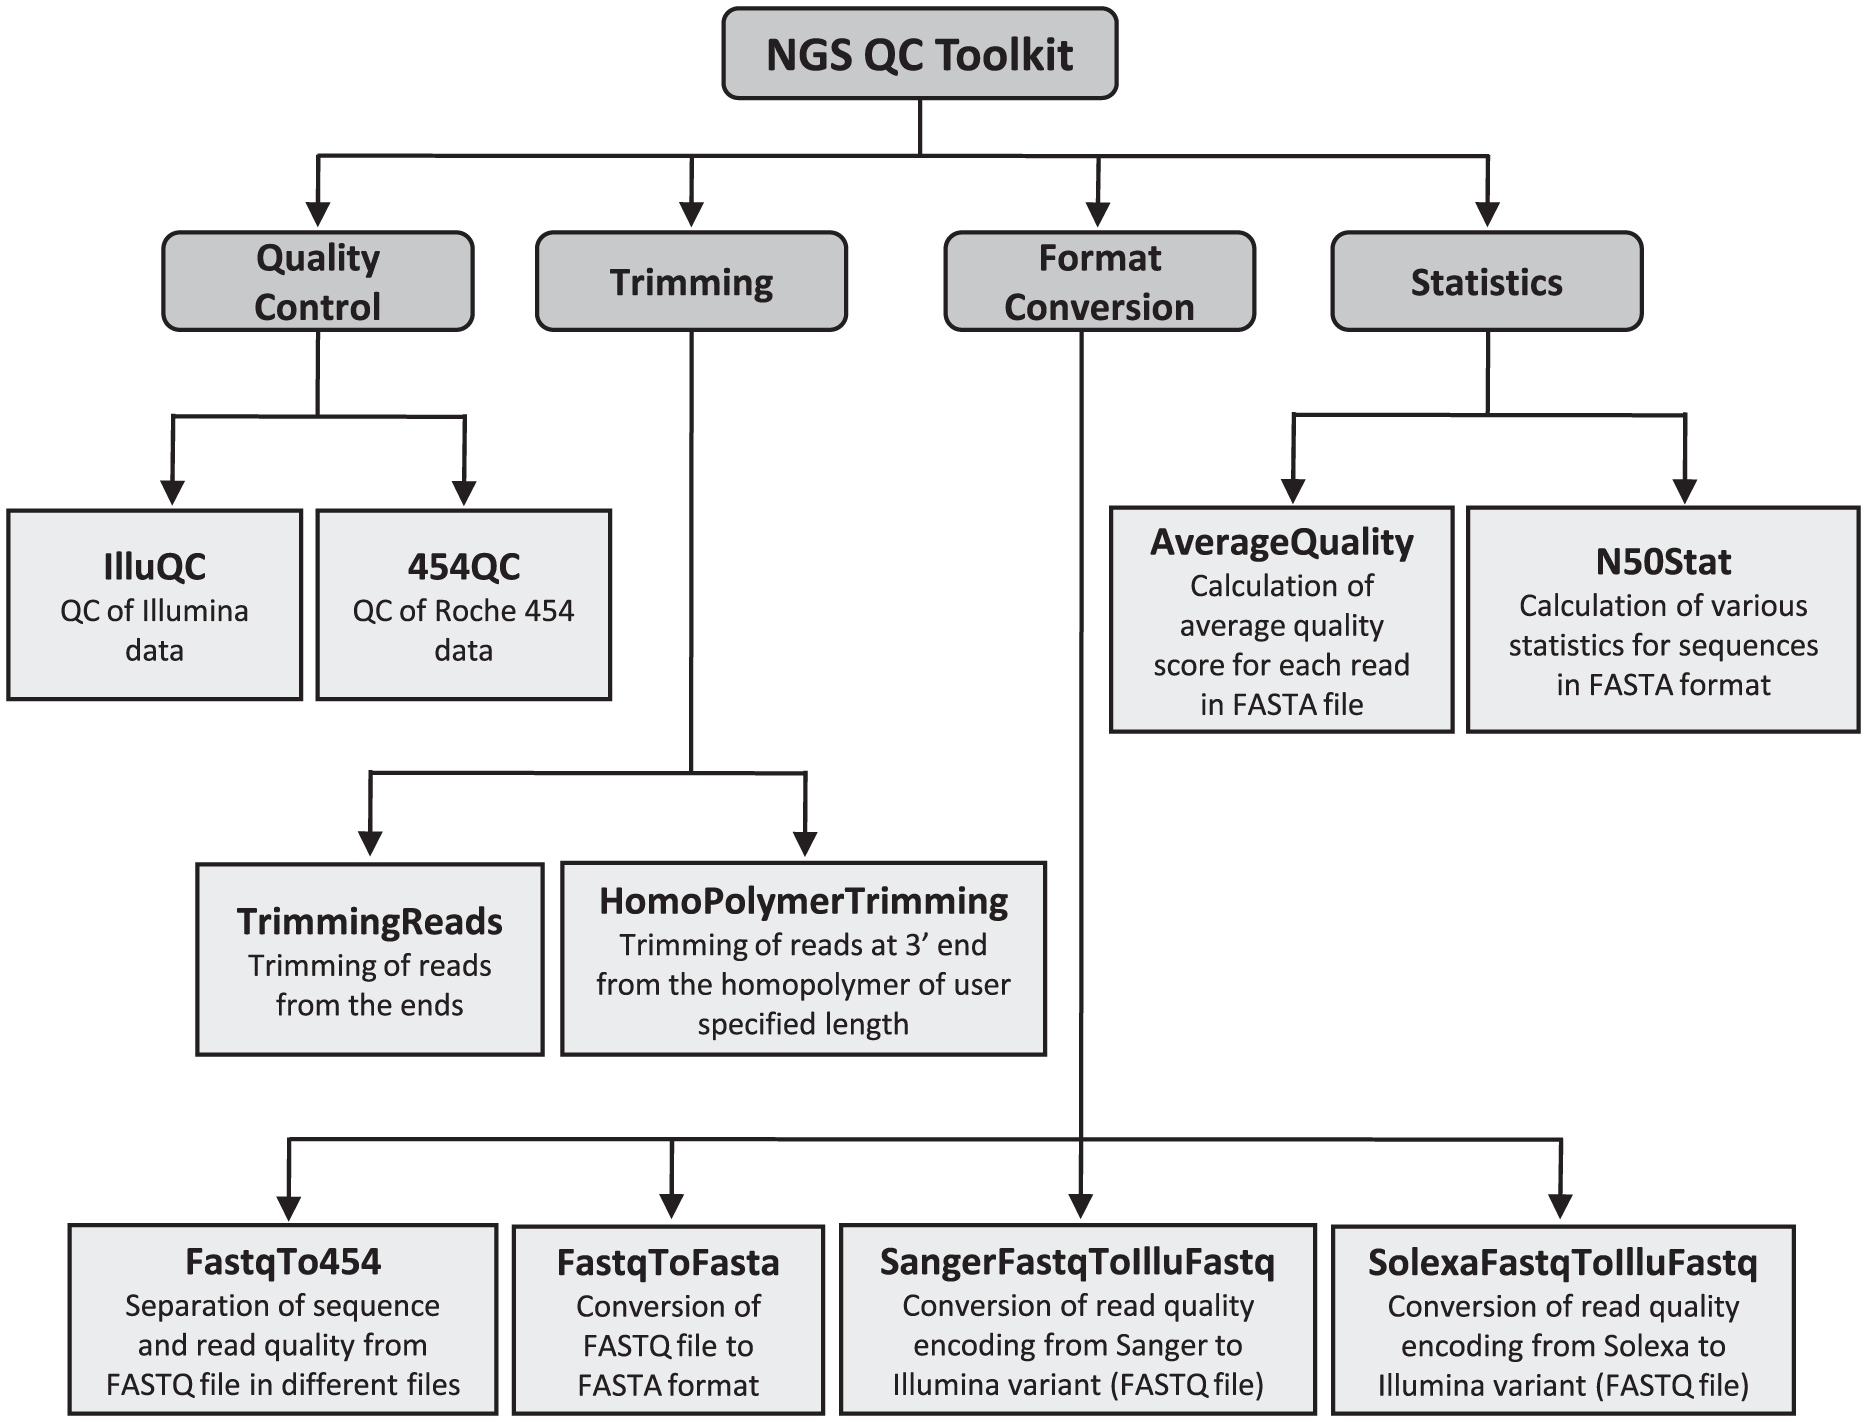
\includegraphics[width=0.8\textwidth]{c2.genomics/qc.ngs.01.png}
  \end{figure}
\end{frame}

\begin{frame}
  \frametitle{基因组学 | 数据分析 | 流程 | 质控 | NGS QC Toolkit}
  \begin{figure}
    \centering
    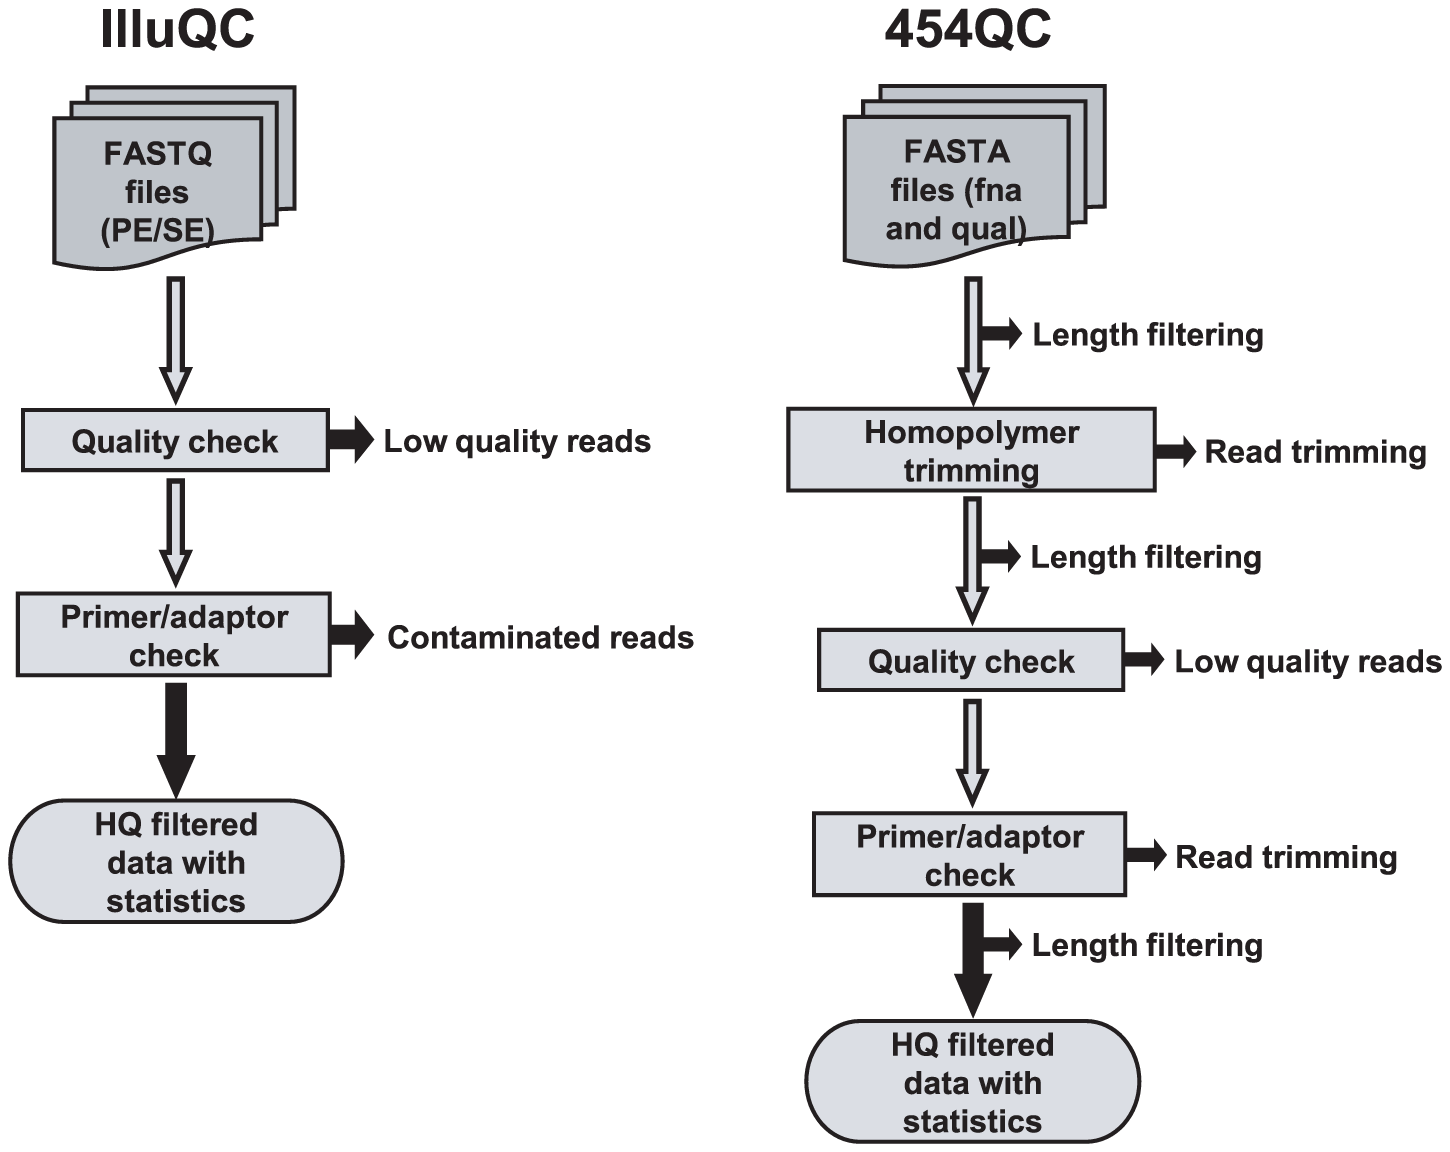
\includegraphics[width=0.8\textwidth]{c2.genomics/qc.ngs.02.png}
  \end{figure}
\end{frame}

\begin{frame}
  \frametitle{基因组学 | 数据分析 | 流程 | 质控 | NGS QC Toolkit}
  \begin{figure}
    \centering
    \includegraphics[width=\textwidth]{c2.genomics/qc.ngs.03.png}
  \end{figure}
\end{frame}

\begin{frame}
  \frametitle{基因组学 | 数据分析 | 流程 | 质控 | NGS QC Toolkit}
  \begin{figure}
    \centering
    \includegraphics[width=\textwidth]{c2.genomics/qc.ngs.04.png}
  \end{figure}
\end{frame}

\begin{frame}
  \frametitle{基因组学 | 数据分析 | 流程 | 质控 | SolexaQA}
  \begin{figure}
    \centering
    \includegraphics[width=\textwidth]{c2.genomics/qc.qa.01.png}
  \end{figure}
\end{frame}

\begin{frame}
  \frametitle{基因组学 | 数据分析 | 流程 | 质控 | SolexaQA}
  \begin{figure}
    \centering
    \includegraphics[width=\textwidth]{c2.genomics/qc.qa.02.png}
  \end{figure}
\end{frame}

\begin{frame}
  \frametitle{基因组学 | 数据分析 | 流程 | 质控 | SolexaQA}
  \begin{figure}
    \centering
    \includegraphics[width=\textwidth]{c2.genomics/qc.qa.03.png}
  \end{figure}
\end{frame}

\begin{frame}
  \frametitle{基因组学 | 数据分析 | 流程 | 预处理}
  \begin{block}{目的}
 manipulating the sequences to produce better mapping results 
  \end{block}
  \pause
  \begin{block}{内容}
    \begin{itemize}
      \item Collapser: Collapsing identical sequences into a single sequence
      \item Clipper: Removing sequencing adapters/linkers
      \item Splitter: Splitting barcode containning multiple samples 
      \item Filter: Filters sequences based on quality
      \item Trimmer: Trims (cuts) sequences based on quality
      \item Formatter: Rename identifiers, Reverse-complement, Mask nucleotides, Convert RNA $\leftrightarrow$ DNA, ...
      \item ...
    \end{itemize}
  \end{block}
\end{frame}

\begin{frame}
  \frametitle{基因组学 | 数据分析 | 流程 | 预处理}
  \begin{figure}
    \centering
    \includegraphics[width=0.7\textwidth]{c2.genomics/pre.01.jpg}
  \end{figure}
\end{frame}

\begin{frame}
  \frametitle{基因组学 | 数据分析 | 流程 | 预处理}
  \begin{figure}
    \centering
    \includegraphics[width=0.9\textwidth]{c2.genomics/pre.02.png}
  \end{figure}
\end{frame}

\begin{frame}
  \frametitle{基因组学 | 数据分析 | 流程 | 预处理 | \textcolor{red}{工具}}
  \begin{block}{FASTX-Toolkit}
    A collection of command line tools for Short-Reads FASTA/FASTQ files preprocessing.
  \end{block}
  \pause
  \begin{block}{PRINSEQ}
    PReprocessing and INformation of SEQuence data. A publicly available tool that is able to filter, reformat and trim your sequences and to provide you summary statistics for your sequence data.
  \end{block}
\end{frame}

\begin{frame}
  \frametitle{基因组学 | 数据分析 | 流程 | 预处理 | FASTX-Toolkit}
  \begin{figure}
    \centering
    \includegraphics[width=0.58\textwidth]{c2.genomics/pre.fastx.cli.01.png}
    \includegraphics[width=0.4\textwidth]{c2.genomics/pre.fastx.galaxy.01.png}
  \end{figure}
\end{frame}

\begin{frame}
  \frametitle{基因组学 | 数据分析 | 流程 | 预处理 | FASTX-Toolkit}
  \begin{figure}
    \centering
    \includegraphics[width=0.75\textwidth]{c2.genomics/pre.fastx.clip.01.png}
  \end{figure}
\end{frame}

\begin{frame}
  \frametitle{基因组学 | 数据分析 | 流程 | 预处理 | PRINSEQ}
  \begin{figure}
    \centering
    \includegraphics[width=0.6\textwidth]{c2.genomics/pre.prinseq.01.png}
  \end{figure}
\end{frame}

\begin{frame}
  \frametitle{基因组学 | 数据分析 | 流程 | 质控与预处理}
  \begin{figure}
    \centering
    \includegraphics[width=0.9\textwidth]{c2.genomics/qc.pre.03.png}
  \end{figure}
\end{frame}

\begin{frame}
  \frametitle{基因组学 | 数据分析 | 流程 | 比对}
  \begin{figure}
    \centering
    \includegraphics[width=0.9\textwidth]{c2.genomics/mapping.01.png}
  \end{figure}
\end{frame}

\begin{frame}
  \frametitle{基因组学 | 数据分析 | 流程 | 比对 | 算法}
  \begin{figure}
    \centering
    \includegraphics[width=0.9\textwidth]{c2.genomics/mapping.02.png}
  \end{figure}
\end{frame}

\begin{frame}
  \frametitle{基因组学 | 数据分析 | 流程 | 比对 | 算法}
  \begin{figure}
    \centering
    \includegraphics[width=0.9\textwidth]{c2.genomics/mapping.03.jpg}
  \end{figure}
\end{frame}

\begin{frame}
  \frametitle{基因组学 | 数据分析 | 流程 | 比对 | 算法}
  \begin{figure}
    \centering
    \includegraphics[width=0.9\textwidth]{c2.genomics/mapping.04.jpg}
  \end{figure}
\end{frame}

\begin{frame}
  \frametitle{基因组学 | 数据分析 | 流程 | 比对 | 算法}
  \begin{figure}
    \centering
    \includegraphics[width=0.9\textwidth]{c2.genomics/mapping.05.jpg}
  \end{figure}
\end{frame}

\begin{frame}
  \frametitle{基因组学 | 数据分析 | 流程 | 比对 | 算法}
  \begin{figure}
    \centering
    \includegraphics[width=0.9\textwidth]{c2.genomics/mapping.06.jpg}
  \end{figure}
\end{frame}

\begin{frame}
  \frametitle{基因组学 | 数据分析 | 流程 | 比对 | 算法 | BWT}
  \begin{figure}
    \centering
    \includegraphics[width=0.9\textwidth]{c2.genomics/mapping.bwt.01.jpg}
  \end{figure}
\end{frame}

\begin{frame}
  \frametitle{基因组学 | 数据分析 | 流程 | 比对 | 算法 | BWT}
  \begin{figure}
    \centering
    \includegraphics[width=\textwidth]{c2.genomics/mapping.bwt.02.jpg}
  \end{figure}
\end{frame}

\begin{frame}
  \frametitle{基因组学 | 数据分析 | 流程 | 比对 | 工具}
  \begin{figure}
    \centering
    \includegraphics[width=0.9\textwidth]{c2.genomics/tool.alignment.01.png}
  \end{figure}
\end{frame}

\begin{frame}
  \frametitle{基因组学 | 数据分析 | 流程 | 比对 | \textcolor{red}{工具}}
  \begin{block}{BWA}
    BWA(Burrows-Wheeler Aligner) is a software package for mapping low-divergent sequences against a large reference genome, such as the human genome.
  \end{block}
  \pause
  \begin{block}{Bowtie}
    \begin{itemize}
      \item Bowtie is an ultrafast, memory-efficient short read aligner.
      \item Bowtie 2 is an ultrafast and memory-efficient tool for aligning sequencing reads to long reference sequences.
    \end{itemize}
  \end{block}
\end{frame}


\begin{frame}
  \frametitle{基因组学 | 数据分析 | 流程 | 比对 | \textcolor{red}{工具}}
  \begin{block}{SOAP}
    SOAP has been in evolution from a single alignment tool to a tool package that provides full solution to next generation sequencing data analysis.
    \begin{itemize}
      \item SOAPaligner/soap2: new alignment tool
      \item SOAPsnp: re-sequencing consensus sequence builder 
      \item SOAPindel: indel finder 
      \item SOAPsv: structural variation scanner
      \item SOAPdenovo: \textit{de novo} shot reads assembler
      \item SOAP3/GPU: GPU-accelerated alignment tool
    \end{itemize}
  \end{block}
\end{frame}

\begin{frame}
  \frametitle{基因组学 | 数据分析 | 流程 | 比对 | BWA}
  \begin{block}{BWA}
     BWA consists of three algorithms: BWA-backtrack, BWA-SW and BWA-MEM.
    \begin{itemize}
      \item BWA-backtrack is designed for Illumina sequence reads up to 100bp, while BWA-SW and BWA-MEM for longer sequences ranged from 70bp to 1Mbp.
      \item BWA-MEM and BWA-SW share similar features such as long-read support and split alignment.
      \item BWA-MEM, which is the latest, is generally recommended for high-quality queries as it is faster and more accurate. BWA-MEM also has better performance than BWA-backtrack for 70-100bp Illumina reads. 
    \end{itemize}
  \end{block}
\end{frame}

\begin{frame}
  \frametitle{基因组学 | 数据分析 | 流程 | 比对 | Bowtie}
  \begin{block}{Bowtie}
 Bowtie aligns short DNA sequences (reads) to the human genome at a rate of over 25 million 35-bp reads per hour. Bowtie indexes the genome with a Burrows-Wheeler index to keep its memory footprint small: typically about 2.2 GB for the human genome (2.9 GB for paired-end).  
  \end{block}
  \pause
  \begin{block}{Bowtie 2}
    Bowtie 2 is particularly good at aligning reads of about 50 up to 100s or 1,000s of characters, and particularly good at aligning to relatively long (e.g. mammalian) genomes. Bowtie 2 indexes the genome with an FM Index to keep its memory footprint small: for the human genome, its memory footprint is typically around 3.2 GB. Bowtie 2 supports gapped, local, and paired-end alignment modes. 
  \end{block}
\end{frame}

\begin{frame}
  \frametitle{基因组学 | 数据分析 | 流程 | 比对 | SOAP}
  \begin{block}{SOAP}
    SOAP is a program for efficient gapped and ungapped alignment of short oligonucleotides onto reference sequences.
  \end{block}
  \pause
  \begin{block}{SOAP2}
    SOAPaligner/soap2 is an updated version of SOAP software for short oligonucleotide alignment. The new program features in super fast and accurate alignment for huge amounts of short reads generated by Illumina/Solexa Genome Analyzer.
  \end{block}
  \pause
  \begin{block}{SOAP3}
    SOAP3 is a GPU-based software for aligning short reads with a reference sequence. It can find all alignments with k mismatches, where k is chosen from 0 to 3. When compared with its previous version SOAP2, SOAP3 can be up to tens of times faster.
  \end{block}
\end{frame}

\begin{frame}
  \frametitle{基因组学 | 数据分析 | 流程 | 提取变异}
  \begin{figure}
    \centering
    \includegraphics[width=0.9\textwidth]{c2.genomics/snp.calling.01.jpg}
  \end{figure}
\end{frame}

\begin{frame}
  \frametitle{基因组学 | 数据分析 | 流程 | 提取变异 | \textcolor{red}{工具}}
  \begin{block}{Samtools}
    Samtools is a suite of programs for interacting with high-throughput sequencing data.
  \end{block}
  \pause
  \begin{block}{GATK}
    Genome Analysis Toolkit: Variant Discovery in High-Throughput Sequencing Data.\\
    The GATK toolkit offers a wide variety of tools with a primary focus on variant discovery and genotyping.
  \end{block}
  \pause
  \begin{block}{VarScan}
    VarScan is a platform-independent software tool developed at the Genome Institute at Washington University to detect variants in NGS data.
  \end{block}
\end{frame}

\begin{frame}
  \frametitle{基因组学 | 数据分析 | 流程 | 提取变异 | Samtools}
  \begin{block}{Samtools}
    Samtools consists of three separate repositories:
    \begin{description}
      \item[Samtools] Reading/writing/editing/indexing/viewing SAM/BAM/CRAM format
      \item[BCFtools] Reading/writing BCF2/VCF/gVCF files and calling/filtering/summarising SNP and short indel sequence variants
      \item[HTSlib] A C library for reading/writing high-throughput sequencing data 
    \end{description}
  \end{block}
\end{frame}

\begin{frame}
  \frametitle{基因组学 | 数据分析 | 流程 | 提取变异 | GATK}
  \begin{figure}
    \centering
    \includegraphics[width=0.9\textwidth]{c2.genomics/snp.calling.gatk.01.png}\\
    \vspace{1em}
    \includegraphics[width=0.9\textwidth]{c2.genomics/snp.calling.gatk.02.png}
  \end{figure}
\end{frame}

\begin{frame}
  \frametitle{基因组学 | 数据分析 | 流程 | 提取变异 | VarScan}
  \begin{block}{VarScan}
    VarScan is a platform-independent mutation caller for targeted, exome, and whole-genome resequencing data generated on Illumina, SOLiD, Life/PGM, Roche/454, and similar instruments. It can be used to detect different types of variation:
    \begin{itemize}
      \item Germline variants (SNPs and indels) in individual samples or pools of samples.
      \item Multi-sample variants (shared or private) in multi-sample datasets (with mpileup).
      \item Somatic mutations, LOH events, and germline variants in tumor-normal pairs.
      \item Somatic copy number alterations (CNAs) in tumor-normal exome data.
    \end{itemize}
  \end{block}
\end{frame}

\begin{frame}
  \frametitle{基因组学 | 数据分析 | 流程 | 注释变异 | \textcolor{red}{工具}}
  \begin{block}{SnpEff}
    Genetic variant annotation and effect prediction toolbox. It annotates and predicts the effects of variants on genes (such as amino acid changes). 
  \end{block}
  \pause
  \begin{block}{ANNOVAR}
    ANNOVAR is an efficient software tool to utilize update-to-date information to functionally annotate genetic variants detected from diverse genomes (including human genome hg18, hg19, hg38, as well as mouse, worm, fly, yeast and many others).
  \end{block}
  \pause
  \begin{block}{SeattleSeq Annotation}
    The SeattleSeq Annotation server provides annotation of SNVs (single-nucleotide variations) and small indels, both known and novel.
  \end{block}
\end{frame}

\begin{frame}
  \frametitle{基因组学 | 数据分析 | 流程 | 注释变异 | SnpEff}
  \begin{block}{Features}
    \begin{itemize}
      \item Supports over 38,000 genomes
      \item Standard ANN annotation format
      \item Cancer variants analysis
      \item GATK compatible (-o gatk)
      \item HGVS notation
      \item Sequence Ontology standardized terms 
    \end{itemize}
  \end{block}
\end{frame}

\begin{frame}
  \frametitle{基因组学 | 数据分析 | 流程 | 注释变异 | ANNOVAR}
  \begin{block}{ANNOVAR}
    Given a list of variants with chromosome, start position, end position, reference nucleotide and observed nucleotides, ANNOVAR can perform:
    {\footnotesize
      \begin{description}
      \item[Gene-based annotation] identify whether SNPs or CNVs cause protein coding changes and the amino acids that are affected.
      \item[Region-based annotation] identify variants in specific genomic regions (conserved regions among 44 species, database of genomic variants, or many other annotations on genomic intervals).
      \item[Filter-based annotation] identify variants that are documented in specific databases, (whether a variant is reported in dbSNP, calculate the SIFT/PolyPhen/... scores, or many other annotations on specific mutations).
      \item[Other functionalities] Retrieve the nucleotide sequence in any user-specific genomic positions in batch, identify a candidate gene list for Mendelian diseases from exome data, and other utilities.
    \end{description}
    }
  \end{block}
\end{frame}

\begin{frame}
  \frametitle{基因组学 | 数据分析 | 流程 | 注释变异 | wANNOVAR}
  \begin{block}{wANNOVAR}
  wANNOVAR is a web server that provides easy and intuitive web-based access to the most popular functionalities of the ANNOVAR software. Users can upload a VCF file and obtain annotated results as tab-delimited or comma-deleted files; in addition, simple variants reduction can be performed to prioritize deleterious variants from the input files. Currently, wANNOVAR supports only human genome annotation.
  \end{block}
\end{frame}

\begin{frame}
  \frametitle{基因组学 | 数据分析 | 流程 | 注释变异 | SeattleSeq}
  \begin{block}{SeattleSeq Annotation}
  This annotation includes:
  \begin{itemize}
    \item dbSNP rs IDs
    \item gene names and accession numbers
    \item variation functions (e.g. missense)
    \item protein positions and amino-acid changes
    \item conservation scores
    \item HapMap frequencies
    \item PolyPhen predictions
    \item clinical association
  \end{itemize}
  \end{block}
\end{frame}

\begin{frame}
  \frametitle{基因组学 | 数据分析 | 流程 | 注释变异 | \textcolor{red}{工具}}
  \begin{block}{SIFT}
    SIFT predicts whether an amino acid substitution affects protein function. SIFT prediction is based on the degree of conservation of amino acid residues in sequence alignments derived from closely related sequences, collected through PSI-BLAST. SIFT can be applied to naturally occurring nonsynonymous polymorphisms or laboratory-induced missense mutations.
  \end{block}
  \pause
  \begin{block}{PolyPhen-2}
    PolyPhen-2 (Polymorphism Phenotyping v2) is a tool which predicts possible impact of an amino acid substitution on the structure and function of a human protein using straightforward physical and comparative considerations.
  \end{block}
\end{frame}

\begin{frame}
  \frametitle{基因组学 | 数据分析 | 流程 | 注释变异 | SIFT}
  \begin{figure}
    \centering
    \includegraphics[width=0.9\textwidth]{c2.genomics/snp.annotation.sift.01.png}
  \end{figure}
\end{frame}

\begin{frame}
  \frametitle{基因组学 | 数据分析 | 流程 | 注释变异 | PolyPhen-2}
  \begin{figure}
    \centering
    \includegraphics[width=0.7\textwidth]{c2.genomics/snp.annotation.polyphen2.01.png}
  \end{figure}
\end{frame}

\begin{frame}
  \frametitle{基因组学 | 数据分析 | 流程 | 可视化 | \textcolor{red}{工具}}
  \begin{block}{Genome Browser}
    interactively visualize genomic data
  \end{block}
  \pause
  \begin{block}{IGV}
    The Integrative Genomics Viewer (IGV) is a high-performance visualization tool for interactive exploration of large, integrated genomic datasets.
  \end{block}
  \pause
  \begin{block}{Tablet}
    Tablet is a lightweight, high-performance graphical viewer for next generation sequence assemblies and alignments.
  \end{block}
  \pause
  \begin{block}{Circos}
    Circos is a software package for visualizing data and information. It visualizes data in a circular layout — this makes Circos ideal for exploring relationships between objects or positions.
  \end{block}
\end{frame}

\begin{frame}
  \frametitle{基因组学 | 数据分析 | 流程 | 可视化 | Genome Browser}
  \begin{figure}
    \centering
    \includegraphics[width=0.9\textwidth]{c2.genomics/vis.gb.01.jpg}
  \end{figure}
\end{frame}

\begin{frame}
  \frametitle{基因组学 | 数据分析 | 流程 | 可视化 | IGV}
  \begin{figure}
    \centering
    \includegraphics[width=0.9\textwidth]{c2.genomics/vis.igv.10.png}
  \end{figure}
\end{frame}

\begin{frame}
  \frametitle{基因组学 | 数据分析 | 流程 | 可视化 | IGV}
  \begin{figure}
    \centering
    \includegraphics[width=0.9\textwidth]{c2.genomics/vis.igv.11.png}
  \end{figure}
\end{frame}

\begin{frame}
  \frametitle{基因组学 | 数据分析 | 流程 | 可视化 | IGV}
  \begin{figure}
    \centering
    \includegraphics[width=0.85\textwidth]{c2.genomics/vis.igv.03.jpg}
  \end{figure}
\end{frame}

\begin{frame}
  \frametitle{基因组学 | 数据分析 | 流程 | 可视化 | IGV}
  \begin{figure}
    \centering
    \includegraphics[width=0.95\textwidth]{c2.genomics/vis.igv.02.png}
  \end{figure}
\end{frame}

\begin{frame}
  \frametitle{基因组学 | 数据分析 | 流程 | 可视化 | GB vs. IGV}
  \begin{figure}
    \centering
    \includegraphics[width=0.9\textwidth]{c2.genomics/vis.gb.igv.01.png}
  \end{figure}
\end{frame}

\begin{frame}
  \frametitle{基因组学 | 数据分析 | 流程 | 可视化 | Tablet}
  \begin{figure}
    \centering
    \includegraphics[width=0.85\textwidth]{c2.genomics/vis.tablet.01.png}
  \end{figure}
\end{frame}

\begin{frame}
  \frametitle{基因组学 | 数据分析 | 流程 | 可视化 | Circos}
  \begin{figure}
    \centering
    \includegraphics[width=0.5\textwidth]{c2.genomics/vis.circos.01.png}
  \end{figure}
\end{frame}

\begin{frame}
  \frametitle{基因组学 | 数据分析 | 流程 | 可视化 | Circos}
  \begin{figure}
    \centering
    \includegraphics[width=0.6\textwidth]{c2.genomics/vis.circos.03.png}
  \end{figure}
\end{frame}

\begin{frame}
  \frametitle{基因组学 | 数据分析 | 流程 | 补遗}
  \begin{figure}
    \centering
    \includegraphics[width=0.9\textwidth]{c2.genomics/tool.other.01.png}
  \end{figure}
\end{frame}

\begin{frame}
  \frametitle{基因组学 | 数据分析 | 流程 | \textcolor{red}{补遗}}
  \begin{block}{Galaxy}
    Galaxy is an open, web-based platform for data intensive biomedical research. Whether on the free public server or your own instance, you can perform, reproduce, and share complete analyses.
  \end{block}
  \pause
  \begin{block}{Picard}
    Picard is a set of command line tools for manipulating high-throughput sequencing (HTS) data and formats such as SAM/BAM/CRAM and VCF.
  \end{block}
\end{frame}

\begin{frame}
  \frametitle{基因组学 | 数据分析 | 流程 | 补遗 | Galaxy}
  \begin{figure}
    \centering
    \includegraphics[width=0.9\textwidth]{c2.genomics/tool.galaxy.00.png}
  \end{figure}
\end{frame}

\begin{frame}
  \frametitle{基因组学 | 数据分析 | 流程 | 补遗 | Galaxy}
  \begin{figure}
    \centering
    \includegraphics[width=0.9\textwidth]{c2.genomics/tool.galaxy.01.png}
  \end{figure}
\end{frame}

\begin{frame}
  \frametitle{基因组学 | 数据分析 | 流程 | 补遗 | Galaxy}
  \begin{figure}
    \centering
    \includegraphics[width=0.9\textwidth]{c2.genomics/tool.galaxy.02.png}
  \end{figure}
\end{frame}

\begin{frame}
  \frametitle{基因组学 | 数据分析 | 流程 | 补遗 | Galaxy}
  \begin{figure}
    \centering
    \includegraphics[width=0.85\textwidth]{c2.genomics/tool.galaxy.03.png}
  \end{figure}
\end{frame}

\begin{frame}
  \frametitle{基因组学 | 数据分析 | 流程 | 补遗 | Galaxy}
  \begin{figure}
    \centering
    \includegraphics[width=0.85\textwidth]{c2.genomics/tool.galaxy.04.png}
  \end{figure}
\end{frame}

\begin{frame}
  \frametitle{基因组学 | 数据分析 | 流程 | 补遗 | Galaxy}
  \begin{figure}
    \centering
    \includegraphics[width=0.8\textwidth]{c2.genomics/tool.galaxy.05.png}
  \end{figure}
\end{frame}

\begin{frame}
  \frametitle{基因组学 | 数据分析 | 流程 | 补遗 | Galaxy}
  \begin{figure}
    \centering
    \includegraphics[width=0.9\textwidth]{c2.genomics/tool.galaxy.06.png}
  \end{figure}
\end{frame}

\begin{frame}
  \frametitle{基因组学 | 数据分析 | 流程 | 补遗 | Galaxy}
  \begin{figure}
    \centering
    \includegraphics[width=0.6\textwidth]{c2.genomics/tool.galaxy.07.png}
  \end{figure}
\end{frame}

\begin{frame}
  \frametitle{基因组学 | 数据分析 | 流程 | 补遗 | Galaxy}
  \begin{figure}
    \centering
    \includegraphics[width=0.9\textwidth]{c2.genomics/tool.galaxy.08.png}
  \end{figure}
\end{frame}

\begin{frame}
  \frametitle{基因组学 | 数据分析 | 流程 | \textcolor{red}{补遗}}
  \begin{block}{bedtools}
    Collectively, the bedtools utilities are a swiss-army knife of tools for a wide-range of genomics analysis tasks. The most widely-used tools enable genome arithmetic: that is, set theory on the genome.
  \end{block}
  \pause
  \begin{block}{BEDOPS}
    BEDOPS is an open-source command-line toolkit that performs highly efficient and scalable Boolean and other set operations, statistical calculations, archiving, conversion and other management of genomic data of arbitrary scale.
  \end{block}
\end{frame}

\begin{frame}
  \frametitle{基因组学 | 数据分析 | 流程 | 补遗 | bedtools}
  \begin{figure}
    \centering
    \includegraphics[width=0.6\textwidth]{c2.genomics/tools.other.bedtools.01.png}
  \end{figure}
\end{frame}

\begin{frame}
  \frametitle{基因组学 | 数据分析 | 流程 | 补遗 | BEDOPS}
  \begin{figure}
    \centering
    \includegraphics[width=0.9\textwidth]{c2.genomics/tools.other.bedops.01.png}
  \end{figure}
\end{frame}

\begin{frame}
  \frametitle{基因组学 | 数据分析 | 流程 | 补遗}
  \begin{figure}
    \centering
    \includegraphics[width=0.9\textwidth]{c2.genomics/tool.other.02.png}
  \end{figure}
\end{frame}

\subsection{应用实例}
\begin{frame}
  \frametitle{基因组学 | 数据分析 | 实例}
  A study published in September 2009 discussed a proof of concept experiment to determine if it was possible to identify causal genetic variants using exome sequencing. They sequenced four individuals with Freeman-Sheldon syndrome (FSS) (OMIM 193700), a rare autosomal dominant disorder known to be caused by a mutation in the gene MYH3. Eight HapMap individuals were also sequenced to remove common variants in order to identify the causal gene for FSS. After exclusion of common variants, the authors were able to identify MYH3, which confirms that exome sequencing can be used to identify causal variants of rare disorders. This was the first reported study that used exome sequencing as an approach to identify an unknown causal gene for a rare mendelian disorder.

  Ng SB, Turner EH, Robertson PD, Flygare SD, Bigham AW, Lee C, Shaffer T, Wong M, Bhattacharjee A, Eichler EE, Bamshad M, Nickerson DA, Shendure J (10 September 2009). "Targeted capture and massively parallel sequencing of 12 human exomes". Nature. 461 (7261): 272–276.
\end{frame}

\begin{frame}
  \frametitle{基因组学 | 数据分析 | 实例}
  Subsequently, another group reported successful clinical diagnosis of a suspected Bartter syndrome patient of Turkish origin. Bartter syndrome is a renal salt-wasting disease. Exome sequencing revealed an unexpected well-conserved recessive mutation in a gene called SLC26A3 which is associated with congenital chloride diarrhea (CLD). This molecular diagnosis of CLD was confirmed by the referring clinician. This example provided proof of concept of the use of whole-exome sequencing as a clinical tool in evaluation of patients with undiagnosed genetic illnesses. This report is regarded as the first application of next generation sequencing technology for molecular diagnosis of a patient.

  hoi M, Scholl UI, Ji W, Liu T, Tikhonova IR, Zumbo P, Nayir A, Bakkaloğlu A, Ozen S, Sanjad S, Nelson-Williams C, Farhi A, Mane S, Lifton RP (10 November 2009). "Genetic diagnosis by whole exome capture and massively parallel DNA sequencing". Proc Natl Acad Sci U S A. 106 (45): 19096–19101. 
\end{frame}

\begin{frame}
  \frametitle{基因组学 | 数据分析 | 实例}
  A second report was conducted on exome sequencing of individuals with a mendelian disorder known as Miller syndrome (MIM\#263750), a rare disorder of autosomal recessive inheritance. Two siblings and two unrelated individuals with Miller syndrome were studied. They looked at variants that have the potential to be pathogenic such as non-synonymous mutations, splice acceptor and donor sites and short coding insertions or deletions. Since Miller syndrome is a rare disorder, it is expected that the causal variant has not been previously identified. Previous exome sequencing studies of common single nucleotide polymorphisms (SNPs) in public SNP databases were used to further exclude candidate genes. After exclusion of these genes, the authors found mutations in DHODH that were shared among individuals with Miller syndrome. Each individual with Miller syndrome was a compound heterozygote for the DHODH mutations which were inherited as each parent of an affected individual was found to be a carrier.

  Sarah B Ng; Kati J Buckingham; Choli Lee; Abigail W Bigham; Holly K Tabor; Karin M Dent; Chad D Huff; Paul T Shannon; Ethylin Wang Jabs; Deborah A Nickerson; Jay Shendure; Michael J Bamshad (2010). "Exome sequencing identifies the cause of a mendelian disorder". Nature Genetics. 42 (1): 30–35. 
\end{frame}

\begin{frame}
  \frametitle{基因组学 | 数据分析 | 实例}
\end{frame}

